% !TEX root = manuscrit.tex

\part{Synthesis of mobile robot protocols}
\label{part:synth}

\chapter[Synchronous Synthesis]{Synthesis of synchronous mobile robot protocols}
\label{chap:synth}

In this chapter, we introduce the use of formal methods for automatic synthesis of autonomous mobile robot algorithms, in the discrete space model. As a case study, we consider the problem of gathering all robots at a particular position, not known beforehand. 
We propose an encoding of the gathering problem in a synchronous execution model as a reachability game, the players being the robot algorithm on one side and the scheduling adversary (that can also dynamically decide robot chirality at every activation) on the other side. Our encoding is general enough to encompass classical execution models for robots evolving on ring-shaped networks, including when several robots are located at the same node and when symmetric situations occur. Our encoding allow us to automatically generate an \emph{optimal} distributed algorithm, in the Fsync model, for three robots evolving on a fixed size ring. The optimality criterion refers to the number of robot moves that are necessary to actually achieve gathering.

\section {Gathering games}
\label{sec:jeux}
In this section we recall classical notions (from~\cite{DBLP:conf/dagstuhl/Mazala01}) related to two-player reachability games, \index{Two-player game} simply called games in the sequel. 

A game is composed of an \emph{arena} and \emph{winning conditions}.

\paragraph{Arena} \index{Arena}An arena for a two-player game is a graph $\arena=(V, E)$ in which the set of vertices
$V=V_p\uplus V_a$ is partitioned into $V_p$, the player locations, and $V_a$
the adversary locations. The set of edges $E\subseteq V\times V$ allows to
define the set of successors of some given vertex $v$, noted $vE=\{v'\in V\mid
(v, v')\in E\}$. %Sometimes the arena is such that $E\subseteq (V_p\times V_a) \cup (V_a\times V_p)$.
In the sequel, we only consider finite arenas.

\paragraph{Plays} \index{Play}To play on an arena, a token is positioned on an initial vertex. Then the token is moved by 
the players from one vertex to 
one of its successors. Each player can move the token only if it is on one of her own vertices. Formally, a play is
a path in the graph. Moreover, we only consider maximal plays:  a 
play is maximal if it is either infinite or finite such that the last vertex of the play has no successor
($\pi=v_0v_1\dots, v_n$, with $v_{n}E=\emptyset$).

\paragraph{Strategies}\index{Strategy}%des \sigma a la place des f...
A strategy for the player determines
to which position she will bring the token whenever it is her turn to play.
To do so, the player takes into account the history of the play, and the current
vertex.
Formally, a strategy for the player is a (partial) function
$\sigma:  V^*\cdot V_p \rightarrow V$ such that, for any sequence (representing the
current history) $w\in V^*$, any $v\in V_p$, $\sigma
(w\cdot v)\in vE$ (\ie the move is possible with respect to the arena). 
A strategy $\sigma$ is \emph{memoryless} if it does not depend on the history. Formally, it means
that for all
$w, w'\in V^*$, for all $v\in V_p$, $\sigma(w\cdot v) = \sigma(w'\cdot v)$. In that case, 
we may simply see the strategy as a mapping $\sigma: V_p\rightarrow V$.

Given a strategy $\sigma$ for the player, a play $\pi=v_0v_1\cdots \in V^\infty$
 is said to be \emph{$\sigma$-consistent} if for all $0<i<| \pi |$, if $v_{i-1}\in V_p$, then $v_i=\sigma
(v_0\cdots v_{i-1})$. Given an initial
vertex $v_{init}$, the \emph{outcome} of a strategy $\sigma$ is the set of plays starting in $v_{init}$
that are $\sigma$-consistent. Formally, given an arena $\arena=(V, E)$, an intial vertex $v_{init}$ and 
a strategy $\sigma: V^*V_p\rightarrow V$, we let $\Outcome(\arena, v_{init}, \sigma)=\{\pi \in V^\infty 
\mid v_0=v_{init}$ and  $\pi$ is a maximal play and is $\sigma$-consistent$\}$.

\paragraph{Winning conditions, winning plays, winning strategies}
 We define the \emph{winning condition} for the player as a subset of the plays $\Win \subseteq V^\infty$.
 Then, a play $\pi$ is \emph{winning} for the player if $\pi\in \Win$. In this work, we focus on the simple
 case of reachability games:  the winning condition is then expressed according to a subset of vertices $T\subseteq V$
 called the \emph{target} by $\Reach(T)=\{\pi=v_0v_1\cdots \in V^\infty\mid \pi$ is maximal and 
 $\exists i,  0\leq i < |\pi|:  v_i \in T\}$. This means that the player
 wins a play whenever the token is brought on a vertex belonging to the set $T$. Once it has happened, the play
 is winning, regardless of the following actions of the adversary.

Given an arena $\arena=(V, E)$, an initial vertex $v_{init}\in V$ and a
winning condition $\Win$, a
\emph{winning strategy} $\sigma$ for the player is a strategy such that
any $\sigma$-consistent play is winning. In other words, a strategy $\sigma$ is winning if
$\Outcome(\arena, v_{init}, \sigma) \subseteq Win$. The player wins the game $(\arena, v_{init}, \Win)$
if she has a winning strategy for $(\arena, v_{init}, \Win)$.
We say that $\sigma$ is winning on a subset $U \subseteq V$ if it is winning
starting from any vertex in $U$: 
$\Outcome(\arena, v, \sigma)\subseteq \Win$ for all $v\in U$.  A subset
$U \subseteq V$ of the vertices is \emph{winning} if there exists
a strategy $\sigma$ that is winning on $U$. The \emph{winning 
region} is the maximal winning set.

\paragraph{Solving a reachability game} \index{Reachability games}
Given an arena $\arena=(V, E)$, a subset $T\subseteq V$, one wants to 
determine the winning region $U\subseteq V$ of the player for $\Reach(T)$, 
and a strategy $\sigma: V^*V_p\rightarrow V$ 
for the player, that is winning on $U$.

\begin{example}
Figure~\ref{fig:synth} represents a reachability two-player game. 
\begin{figure}[htbp]
\centering 
\begin{tikzpicture} [thick, node distance= 6em, >=stealth, ->, scale=0.8, transform shape] 
\node[rectangle, draw, text centered](P1) {P1};
\node[rectangle, draw, text centered, left of =P1](P4){P4};
\node[circle, draw, text centered, above of = P1] (E1) []{O1};
\node[rectangle, draw, text centered, right of = E1](P2) {P2};
\node[circle, draw, text centered, above right= 1em and 4em of P1] (E3) []{O3};
\node[circle, draw, text centered, below right= 1em and 4em of P1] (E2) []{O2};
\node[rectangle, draw, text centered, above right = 1em and 4em of E2, fill=gray!60](P3) {P3};

\path (P1) edge[] (E1) 
         (P1) edge[] (P4)
	(E1) edge[] (P2) 
	(P2) edge[bend right] (E1) 
	(P1) edge[] (E2)
	(E1) edge [] (E3)
	(E2) edge[] node{} (P3)
	(P3) edge[] (E3)
	(E3) edge[] (P1)
	(P4) edge[loop above] (P4);
	
\end{tikzpicture} 
\caption{A two player game with a reachability objective.} 
\label{fig:synth}
\end{figure}
Player vertices are here represented by rectangles and adversary vertices by circles. 
The winning condition is $\Reach(\{P3\})$. 
From P2 the player has no winning strategy, since from O1 the adversary
can always bring the game back to P2, producing an infinite loop that never goes to the target. 
From P1 a (memoryless) winning strategy is to go to O2.
The winning region of the player is $\{P1, P3\}$.
\end{example}

We recall now a well-known result on reachability games~\cite{MartinBorelDeterminacy}: 
%stating that one does not need memory to win a reachability game: 
\begin{theorem} \label{th: memoryless}The winning region for the player in a reachability
game can be computed in linear time in the size of the arena. Moreover, from any location, the player
has a winning strategy if and only if she has a memoryless winning strategy.
\end{theorem}%The theorem obviously only make sense if the arena is finite (this is not require previously) -> in linear time:  according to the size of the arena







\section {Synthesis for synchronous robots}
		\subsection {Arena construction}
		\label{sub:synth}
We build an arena for a reachability game, such that the player has a winning strategy 
if and only if one can design an algorithm for synchronous robots to gather on a single node, 
starting from any configuration. We consider the arena $\Agather=(V_p\uplus V_a, E)$, 
where:  
\begin{itemize}
\item the set of player locations is $V_p= (\ObsClass)$, the set of equivalence classes of observations (see Definition~\ref{def:obs} in Chapter~\ref{chap:model}), 
\item the set of adversary locations 
is $V_a= \Obs \times \Actions^k$, with $\Actions=\{ \clockwise, \counterclockwise, \?, \still \}$  the set of actions as defined in~\ref{subsub:move}. 
\end{itemize}
The size of the arena is thus linear in $n$ and exponential in $k$.
The edge relation $E$ is detailed in the rest of the subsection and will ensure a strict alternation between the two players:  $E\subseteq (V_p\times V_a) \cup (V_a\times V_p)$.

\subsubsection{Edges from $V_p$ to $V_a$}
From a player location, representing an equivalence class of observations, 
the play continues on an adversary location memorizing the different movements
decided by each robot. Such a move is possible if, in a given equivalence class
of observations, the robots with the same view take the same decision. Recall that an algorithm 
$\mathcal{S}$ is given by a decision function (see Definition~\ref{def:decisionFunction} in Chapter~\ref{chap:model}).
\bigskip


We now define the edge relation from a player location to an adversary
location. For $v\in V_p$, recall that we can consider the canonical configuration $c_o$ for $o=\rep(v)$. 
Then $(v, v')\in E$ with $v'=\bigl (o, (a_1, \dots, a_k)\bigr )$ if and only if there exists 
a decision function $\partial$ such that $a_i=\dec(\view(r_i, c_o))$ for all $i$ in  $[1.. k]$.


\subsubsection{Edges from $V_a$ to $V_p$}
The moves of the adversary lead the game into the configuration of 
the system resulting from the application of the decisions of all robots. 
If a robot decides to move, but is disoriented, then the adversary
chooses the actual move (\clockwise{} or \counterclockwise). 
The next configuration is then determined by the actions chosen 
and the decisions taken by the adversary, defined as a $k$-tuple of movements
$m= (m_i)_{1\leq i \leq k} \in (\Actions \setminus \{\?\})^k$.

Let $r$ be a robot and let $c'$ be the configuration resulting from the move $m$ applied
to configuration $c$. We write $\obs(r, c') = \obs(r, c) \oplus m$ the corresponding 
observation. The next result states that the equivalence classes are consistent 
with equivalent movements of the robots. 
 \begin{proposition}
 \label{prop: bisim}
 Let $c \Cequiv c'$ be two equivalent configurations, and let $o$ and 
 $o'$ be observations of $c$ and $c'$ respectively.
 Then, for any move $m = (m_1, \dots, m_k)\in(\Actions \setminus \{\?\})^k$, there  
 exists $m' = (m'_1, \dots, m'_k)\in(\Actions \setminus \{\?\})^k$
  such that  $o\oplus m \equiv o'\oplus m'$.
 \end{proposition}
  \begin{proof}
 Let $c, c' \in \Config$ with
 $c'\Cequiv c$ and let $o, o' \in \Obs$ be observations of $c$ and $c'$ respectively. 
 For a  move $m=(m_i)_{1\leq i \leq k}\in (\Actions \setminus \{\?\})^k$ from $c$, 
 we define the move $m'$ that will represent the same decisions, on 
 configuration $c'$. Thanks to Proposition~\ref{prop:Oequ}, 
 we know that $o$ and $o'$ are in the same equivalence class for $\Oequiv$, hence 
if $o=\{(f_1, \cdots, f_k), (f_k, \cdots, f_1)\}$ then $o'=\{(f_i, \dots, f_k, f_1, \dots, f_{i-1}), (f_{i-1}, \dots, f_1, f_k, \dots, f_{i})\}$ 
for some $i$, $1\leq i\leq k$.
Now, ordering the two tuples of $o'$ in lexicographical order, we consider two cases.
If $(f_i, \dots, f_k, f_1, \dots, f_{i-1})$ is the smallest observation, then
 $m'_j=m_{(i+j-1)}$ for all $1\leq j\leq k$. Otherwise,  for all $1\leq j\leq k$:  
 $$m'_j= \begin{cases}
 \clockwise &\textrm{if }m_{i-j}=\counterclockwise\\
 \counterclockwise &\textrm{if }m_{i-j}=\clockwise\\
 \still &\textrm{if }m_{i-j}=\still
 \end{cases}$$
  We have $o\oplus m \equiv o'\oplus m'$.
 \end{proof}
 
We now define $v$-consistent moves where the adversary in some vertex $v$ resolves 
all the $\?$ actions by choosing in which directions disoriented robots will move.
\begin{definition}\label{def:vCo}
For a state $v=(o, (a_1, \dots, a_k))\in V_a$, a move $m = (m_1, \dots, m_k)\in(\Actions \setminus \{\?\})^k$
 is \emph{$v$-consistent} if:  
\begin{itemize}
\item for all $1\leq i\leq k$ such that $a_i\neq\disoriented$, $m_i=a_i$, 
\item for all $1\leq i\leq k$ such that $a_i=\disoriented$, $m_i\neq\still$.
\end{itemize}
\end{definition}


The edge relation from an adversary location 
to a player location is then defined by:  for $v=(o, (a_1, \dots, a_k))\in V_a$, and $v' \in V_p$, 
the edge $(v, v')$ belongs to $E$ if and only if there exists a $v$-consistent 
move m such that $v'=\equivclass{o\oplus m}$.

The Figure~\ref{fig:Agather} represents a part of the gathering arena for 4 robots on a ring of size 12.
\begin{figure}
\begin{tikzpicture} [thick, node distance= 14em, >=stealth, ->, scale=0.7, transform shape, text centered] 
\node[circle, minimum size =6.5em, draw, thick] (C){};
\node[rectangle, rounded corners=5pt, draw, below = 0.75em of C](W) {{$\equivclass{(-1, 1, 7, 1)}$}};
\foreach \i in {0, ..., 11}
\node[circle, minimum size =0.75em, draw, thick, fill=white]at(\i*30: 1.35)(W\i){};
\node[circle, minimum size =1em, draw, thick, fill=black]at(3*30: 1.35)(N1){};
\node[circle, minimum size =1em, draw, thick, fill=black]at(3*30: 1.7)(N2){};
\node[circle, minimum size =1em, draw, thick, fill=black]at(1*30: 1.35)(N3){};
\node[circle, minimum size =1em, draw, thick, fill=black]at(5*30: 1.35)(N4){};


\node[ellipse, draw, rounded corners=5pt, below  = 12.5 em of W](T1){(-1, 1, 7, 1), (D, D, I, I)};
\node[circle, minimum size =6.5em, draw, thick, below of =C](CT1){};
\foreach \i in {0, ..., 11}
\node[circle, minimum size =1em, draw, thick, fill=white, below of =W\i](T1\i){};
\node[circle, minimum size =1em, draw, thick, fill=black, below of =N1](N11){};
\node[circle, minimum size =1em, draw, thick, fill=black, below of =N2](N21){};
\node[circle, minimum size =1em, draw, thick, fill=black, below of =N3](N31){};
\node[circle, minimum size =1em, draw, thick, fill=black, below of =N4](N41){};


\node[ellipse, rounded corners=5pt, above = 11.25em of W, draw, node distance = 14em](T0){(-1, 1, 7, 1), (I, I, I, I)};
\node[circle, minimum size =6.5em, draw, thick, above of =C](CT0){};
\foreach \i in {0, ..., 11}
\node[circle, minimum size =1em, draw, thick, fill=white, above of =W\i](T0\i){};
\node[circle, minimum size =1em, draw, thick, fill=black, above of =N1](N10){};
\node[circle, minimum size =1em, draw, thick, fill=black, above of =N2](N20){};
\node[circle, minimum size =1em, draw, thick, fill=black, above of =N3](N30){};
\node[circle, minimum size =1em, draw, thick, fill=black, above of =N4](N40){};


\node[circle, minimum size =6.5em, draw, thick, above right = 3em and  7.75em of C](CT3){};
\foreach \i in {0, ..., 11}
\node[circle, minimum size =1em, draw, thick, fill=white, above right = 7em and  11.5em of W\i](T3\i){};
\node[circle, minimum size =1em, draw, thick, fill=black, above right = 7em and 11.5em of N1](N13){};
\node[circle, minimum size =1em, draw, thick, fill=black, above right = 7em and 11.5em of N2](N23){};
\node[circle, minimum size =1em, draw, thick, fill=black, above right = 7em and 11.5em of N3](N33){};
\node[circle, minimum size =1em, draw, thick, fill=black, above right = 7em and 11.5em of N4](N43){};
\node[ellipse, rounded corners=5pt, below = 0.25em of T39, draw](T3){(-1, 1, 7, 1), (D, D, F, F)};

\node[circle, minimum size =6.5em, draw, thick, below right = 3em and 7.75 em of C](CT4){};
\foreach \i in {0, ..., 11}
\node[circle, minimum size =1em, draw, thick, fill=white, below right = 7em and 11.5em of W\i](T4\i){};
\node[circle, minimum size =1em, draw, thick, fill=black, below right = 7em and 11.5em of N1](N14){};
\node[circle, minimum size =1em, draw, thick, fill=black, below right = 7em and 11.5em of N2](N24){};
\node[circle, minimum size =1em, draw, thick, fill=black, below right = 7em and 11.5em of N3](N34){};
\node[circle, minimum size =1em, draw, thick, fill=black, below right = 7em and 11.5em of N4](N44){};
\node[ellipse, rounded corners=5pt, below = 0.25em of T49, draw](T4){(-1, 1, 7, 1), (I, I, F, F)};


\node[circle, minimum size =6.5em, draw, thick, above left = 3em and 7.75 em of C](CT5){};
\foreach \i in {0, ..., 11}
\node[circle, minimum size =1em, draw, thick, fill=white, above left = 7em and 11.5em of W\i](T5\i){};
\node[circle, minimum size =1em, draw, thick, fill=black, above left = 7em and 11.5em of N1](N15){};
\node[circle, minimum size =1em, draw, thick, fill=black, above left = 7em and 11.5em of N2](N25){};
\node[circle, minimum size =1em, draw, thick, fill=black, above left = 7em and 11.5em of N3](N35){};
\node[circle, minimum size =1em, draw, thick, fill=black, above left = 7em and 11.5em of N4](N45){};
\node[ellipse, rounded corners=5pt, below = 0.25em of T59, draw](T5){(-1, 1, 7, 1), (D, D, B, B)};


\node[circle, minimum size =6.5em, draw, thick, below left = 3em and 7.75 em of C](CT6){};
\foreach \i in {0, ..., 11}
\node[circle, minimum size =1em, draw, thick, fill=white, below left = 7em and 11.5em of W\i](T6\i){};
\node[circle, minimum size =1em, draw, thick, fill=black, below left = 7em and 11.5em of N1](N16){};
\node[circle, minimum size =1em, draw, thick, fill=black, below left = 7em and 11.5em of N2](N26){};
\node[circle, minimum size =1em, draw, thick, fill=black, below left = 7em and 11.5em of N3](N36){};
\node[circle, minimum size =1em, draw, thick, fill=black, below left = 7em and 11.5em of N4](N46){};
\node[ellipse, rounded corners=5pt, below = 0.25em of T69, draw](T6){(-1, 1, 7, 1), (I, I, B, B)};

%suite de CT3
\node[circle, minimum size =6.5em, draw, thick, above right = 7.1em and  7.5em of CT3](CT3A){};
\foreach \i in {0, ..., 11}
\node[circle, minimum size =1em, draw, thick, fill=white, above right = 11em and  11.5em of T3\i](T3A\i){};
\node[circle, minimum size =1em, draw, thick, fill=black, above right = 11em and 11.5em of T32](N13A){};
\node[circle, minimum size =1em, draw, thick, fill=black, above right = 11em and 11.5em of T34](N23A){};
\node[circle, minimum size =1em, draw, thick, fill=black, above right = 12.5em and 10em of T34](N33A){};
\node[circle, minimum size =1em, draw, thick, fill=black, above right = 11.75em and 10.75em of T34](N43A){};
\node[rectangle, rounded corners=5pt, below = 0.25em of T3A9, draw](T3A){$\equivclass{(-1, -1, 1, 9)}$};
\node[circle, minimum size =6.5em, draw, thick, right = 5.75em of CT3](CT3B){};
\foreach \i in {0, ..., 11}
\node[circle, minimum size =1em, draw, thick, fill=white, right = 11.5em of T3\i](T3B\i){};
\node[circle, minimum size =1em, draw, thick, fill=black, right = 11.5em of T32](B1){};
\node[circle, minimum size =1em, draw, thick, fill=black, above right = 0em and 0em of B1](NB23){};
\node[circle, minimum size =1em, draw, thick, fill=black, right = 11.5em of T34](NB33){};
\node[circle, minimum size =1em, draw, thick, fill=black, above left = 0em and 0em of NB33](NB43){};
\node[rectangle, rounded corners=5pt, below = 0.25em of T3B9, draw](T3B){$\equivclass{(-1, 1, -1, 9)}$};


%suite de CT4
\node[circle, minimum size =6.5em, draw, thick, right = 5.75em of CT4](CT4bis){};
\foreach \i in {0, ..., 11}
\node[circle, minimum size =1em, draw, thick, fill=white, right = 11.5em of T4\i](T4B\i){};
\node[circle, minimum size =1em, draw, thick, fill=black, right = 11.5em of T42](TB42){};
\node[circle, minimum size =1em, draw, thick, fill=black, right = 11.5em of T43](TBB){};
\node[circle, minimum size =1em, draw, thick, fill=black, above = 0em of TBB](NB43){};
\node[circle, minimum size =1em, draw, thick, fill=black, right = 11.5em of T44](NB44){};
\node[rectangle, rounded corners=5pt, below = 0.25em of T4B9, draw](T4B){$\equivclass{(-1, 0, 9, 0)}$};

%suite de CT5
\node[circle, minimum size =6.5em, draw, thick, above left = 7.1em and  7.5em of CT5](CT5A){};
\foreach \i in {0, ..., 11}
\node[circle, minimum size =1em, draw, thick, fill=white, above left = 11em and  11.5em of T5\i](T5A\i){};
\node[circle, minimum size =1em, draw, thick, fill=black, above left = 11em and 11.5em of T50](N50A){};
\node[circle, minimum size =1em, draw, thick, fill=black, above left = 11em and 11.5em of T52](N52A){};
\node[circle, minimum size =1em, draw, thick, fill=black, above right = 0em and 0em of N52A](N52AA){};
\node[circle, minimum size =1em, draw, thick, fill=black, above left = 11em and 11.5em of T56](N56A){};
\node[rectangle, rounded corners=5pt, below = 0.25em of T5A9, draw](T5A){$\equivclass{(-1, 1, 5, 3)}$};
\node[circle, minimum size =6.5em, draw, thick, left = 5.75em of CT5](CT5B){};
\foreach \i in {0, ..., 11}
\node[circle, minimum size =1em, draw, thick, fill=white, left = 11.5em of T5\i](T5B\i){};
\node[circle, minimum size =1em, draw, thick, fill=black, left = 11.5em of T50](N50B){};
\node[circle, minimum size =1em, draw, thick, fill=black, left = 11.5em of T52](NB52){};
\node[circle, minimum size =1em, draw, thick, fill=black, left = 11.5em of T54](NB54){};
\node[circle, minimum size =1em, draw, thick, fill=black, left = 11.5em of T56](NB56){};
\node[rectangle, rounded corners=5pt, below = 0.25em of T5B9, draw](T5B){$\equivclass{(1, 1, 1, 5)}$};


%suite de CT6
\node[circle, minimum size =6.5em, draw, thick, left = 5.75em of CT6](CT6bis){};
\foreach \i in {0, ..., 11}
\node[circle, minimum size =1em, draw, thick, fill=white, left = 11.5em of T6\i](T6B\i){};
\node[circle, minimum size =1em, draw, thick, fill=black, left = 11.5em of N26](TB26){};
\node[circle, minimum size =1em, draw, thick, fill=black, left = 11.5em of N16](NB16){};
\node[circle, minimum size =1em, draw, thick, fill=black, left = 11.5em of T60](NB60){};
\node[circle, minimum size =1em, draw, thick, fill=black, left = 11.5em of T66](NB66){};
\node[rectangle, rounded corners=5pt, below = 0.25em of T6B9, draw](T6B){$\equivclass{(-1, 2, 5, 2)}$};

%suite de T1
\node[circle, minimum size =6.5em, draw, thick, below right = 3em and 7.75 em of CT1](CT1A){};
\foreach \i in {0, ..., 11}
\node[circle, minimum size =1em, draw, thick, fill=white, below right = 7em and 11.5em of T1\i](T1A\i){};
\node[circle, minimum size =1em, draw, thick, fill=black, below right = 7em and 11.5em of T11](T11A){};
\node[circle, minimum size =1em, draw, thick, fill=black, below right = 7em and 11.5em of T12](T12A){};
\node[circle, minimum size =1em, draw, thick, fill=black, below right = 7em and 11.5em of T14](T14A){};
\node[circle, minimum size =1em, draw, thick, fill=black, below right = 7em and 11.5em of T15](T15A){};
\node[rectangle, rounded corners=5pt, below = 0.25em of T1A9, draw](T1A){$\equivclass{(0, 1, 0, 7)}$};

\node[circle, minimum size =6.5em, draw, thick, below left = 3em and 7.75 em of CT1](CT1B){};
\foreach \i in {0, ..., 11}
\node[circle, minimum size =1em, draw, thick, fill=white, below left = 7em and 11.5em of T1\i](T1B\i){};
\node[circle, minimum size =1em, draw, thick, fill=black, below left = 7em and 11.5em of T11](T11B){};
\node[circle, minimum size =1em, draw, thick, fill=black, below left = 7em and 11.5em of T14](T12B){};
\node[circle, minimum size =1em, draw, thick, fill=black, above left = 0em and 0em of T12B](T12BB){};
\node[circle, minimum size =1em, draw, thick, fill=black, below left = 7em and 11.5em of T15](T15B){};
\node[rectangle, rounded corners=5pt, below = 0.25em of T1B9, draw](T1B){$\equivclass{(-1, 0, 7, 2)}$};
	
	
\path		(N2.north) edge[] (T0.south)
	 	(W.south) edge[] (N21.north)
		(W2) edge[] (T37)
		(W11) edge[] (T44)
		(W4) edge[] (T511)
		(W7) edge[] (T62)
		(T66) edge[] (T6B0)
		(T56) edge[] (T5B0)
		(T54) edge[] (T5A11)
		(T30) edge[] (T3B6)
		(T32) edge[] (T3A7)
		(T40) edge[] (T4B6)
		(T17) edge[] (T1B2)
		(T111) edge[] (T1A4)
		;%[bend right=75, looseness=1.5] (N2.north east);

\end{tikzpicture} 
\caption{A part of the gathering arena for 4 robots in a 12 nodes ring.} 
\label{fig:Agather}
\end{figure}


\bigskip

In this context, gathering can be reformulated as follows: \\
Let $v_T=\equivclass{(-1, \cdots, -1, n-1), (n-1, -1, \cdots, -1)}\in V_p$ 
be the equivalence class 
of all configurations corresponding to all robots positioned on a single node.
For the game on $\Agather$ with winning condition $\Reach(\{v_T\})$, the winning region corresponds
 exactly to the set of configurations from which robots can achieve the gathering. 
 
We must show now that solving this reachability game 
amounts to automatically synthesizing a deterministic algorithm achieving the gathering for this system.
Let $\mathcal{S}$ be an algorithm given by its decision function $\dec_\mathcal{S}$.
The notion of consistency is adapted to $\mathcal{S}$ as follows:  
for a configuration $c\in\Config$ and a corresponding observation $o\in \Obs$, 
$m \in (\Actions \setminus \{\?\})^k$ is a $(\mathcal{S}, c)$-consistent move 
if it is a $v$-consistent move for $v=(o, (a_1, \dots, a_k))$ with 
$a_i=\dec_\mathcal{S}(\view(r_i, c))$, $1\leq i \leq k$. We denote by $M(\mathcal{S}, c)$ the set of all $(\mathcal{S}, c)$-consistent moves.\\
 Let $c, c'$ be two configurations, and let $o$ and $o'$ be observations such that $o = \obs(r, c)$ and $o'=\obs(r, c')$
 for some robot $r$. We denote by $c\xrightarrow{m} c'$ 
 the application to configuration $c$ of the move $m$, where $m$ is $(\mathcal{S}, c)$-consistent,  
 leading to configuration $c'$, defined by:  $o' = o \oplus m$.
 
For a configuration $c$, we note $\suc(\mathcal{S}, c)$ 
the set of configurations produced by applying $M(\mathcal{S}, c)$ on $c$, 
more formally:    $$\suc(\mathcal{S}, c) = \{ c' \mid \exists m \in M(\mathcal{S}, c) \st c\xrightarrow{m} c' \}.$$
Proposition~\ref{prop: bisim} implies that, for two equivalent configurations $c\Cequiv c'$, 
$\suc(\mathcal{S}, c)  = \suc(\mathcal{S}, c')$.

The next result gives the correspondence between algorithms and winning strategies in the reachability game.
\begin{theorem}\label{th: correctness}
There exists an algorithm which achieves gathering if and only if there exists a memoryless winning strategy 
for the reachability game $\Agather$ with winning condition $\Reach(\{v_T\})$.
\end{theorem}

\begin{proof}
We first show that if some algorithm $\mathcal{S}$ achieves gathering 
then we can build a winning strategy $\sigma: V_p\rightarrow V_a$. 
Conversely we show that given a winning region and a memoryless strategy, one can 
define a unique algorithm for the robots.

From $\mathcal{S}$ we construct the memoryless strategy $\sigma$ defined for any 
$v \in V_p$ by:  $$\sigma(v) = 
(rep(v), (a_1, \dots, a_k)) \textrm{ with } a_i=\dec_\mathcal{S}(\view(r_i, c_{rep(v)})), 1\leq i \leq k.$$
We now have to prove that if $\mathcal{S}$ achieves the gathering then $\sigma$ is winning.
Our interest is on the plays in the $\Outcome$ of $\sigma$:  these plays are $\sigma$-consistent
and any edge $(v, v') \in V_a \times V_p$ in these plays results from a $v$-consistent move: 
For such an edge $(v, v')$, let $c$ be the configuration in $v$, with observation $o$, there exists a $v$-consistent 
move $m$ such that $v'= \equivclass{o'}$, with $o' = o \oplus m $. 
Since $m$ is also $(\mathcal{S}, c)$-consistent, then 
$c' \in \suc(\mathcal{S}, c)$ 
and thus, any configuration from which the algorithm ensures gathering is winning for the game.

Conversely, let $W$ be the winning region, and let $\sigma$ be a (memoryless, from 
Theorem~\ref{th: memoryless}) winning strategy. 
For a configuration $c \in \Config$, $o$ a corresponding observation, 
assume that the strategy is defined by:   $\sigma(\equivclass{o}) = 
(rep(\equivclass{o}), (a_1, \dots, a_k))$.  Then, we define a unique algorithm $\mathcal{S}$ 
by extracting the decision function underneath the strategy as follows:   
$\dec_\mathcal{S}(\view(r_i, c))= a_i$, for all robots $r_i \in \Rob$. 
%Thanks to our arena construction:   two robots on a same tower has the same view, 
%two symmetrical robots have the same view and disoriented robots have only two 
%possible actions:  $\?$ and $\Idle$.
We now show that this algorithm achieves gathering from any configuration $c$ such that its 
observation class $\equivclass{o}$ belongs to  $W$.
%The robots implementing $\mathcal{S}$ achieve the gathering from $c$ if
%for all $c' \in \suc(\mathcal{S}, c)$ the plays $\equivclass{\obs(r, c)} $ is f-consistent since f is a winning strategy. 
Let $c'$ be a configuration in $\suc(\mathcal{S}, c)$, then there exists a 
$(\mathcal{S}, c)$-consistent move $m \in M(\mathcal{S}, c)$ such that $c\xrightarrow{m} c' $. 
 %Since $m$ is also consistent with $f_\mathcal{S}$
  %such that $\obs(r, c) \oplus m = \obs(r, c')=o'$. 
 For all succession of configurations 
$c\xrightarrow{m} c'\xrightarrow{} \dots$ obtained by successive applications of the algorithm, 
we have a corresponding play %$(\equivclass{\obs(r, c)})v(\equivclass{o'})\dots$ 
that is $\sigma$-consistent, in the game. 
Since $\equivclass{o}$ is a winning position, the play is winning and $\mathcal{S}$
achieves gathering. 
\end{proof}

In the following subsection we explain in details how the robot moves have been implemented. 
%pas forcément à lire pour un reader ne voulant pas encoder nos robot moves 
In particular the  $o \oplus m$ notation is defined explicitely
 here.

%%%%%%%%%%%%%%%%%%%%%%%%%%%%%%%%
\subsection {Implementation details}
\label{subsec:implemSync}
%%%%%%%%%%%%%%%%%%%%%%%%%%%%%%%%

%\todo{ici on doit avoir les mouvements inverse car on est plus sur les mouvements 
%des robots mais sur les mouvements et leur efficience sur la configuration
%dans la partie asynchrone dire que ça doit être fait a chaque étape ...}

For efficiency reasons, our implementation does not handle configurations but only observations. 
More precisely we only work on the smallest $k$-tuple in $\mathcal{F}$ of an observation, 
from which we must recover the relevant information to perform robot moves.
Recall (from Subsection \ref{subsubsec:obs}) that from an observation class
$\obs \in \ObsClass$, we extract an observation $rep(\obs) = o =
\{F, \tilde{F}\}$ with $F=(f_1, \dots, f_k)$ in $\mathcal{F}$ minimal among all tuples in $\obs$.
We associate with $o$ a canonical configuration 
$c_o$ defined by $c_o(r_1)=0$, $c_o(r_2)=f_1+1, \dots, 
 c_o(r_k) = \Sigma_{i=1}^k f_i \plusN k$ 
where the robot $r_i$ is at distance $f_i$ of robot $r_{i \plusK 1}$.  

 Recall that a robot movement in $\Front, \Back, \Idle$ is given according to 
 the robot minimal view (see the paragraph~\ref{subsub:move}). 
 When a robot $r_i$ moves, it modifies the distances $f_i$ and $f_{i-1}$ 
 (increasing one of these two distances by one, and  decreasing by one 
 the other). Formally, the effect on an observation of a  configuration, 
 of any movement $m_i$ of robot $r_i$ can be described by a mapping 
 $\varepsilon:   \{1, \ldots, k\} \times \{\Front, \Back, \Idle\} \times F \to \{-1, 0, 1\}^k$.
 This mapping denotes the translated moves 
 that permit to apply real movements on the observations class and 
 is defined by:   \begin{itemize}
 \item If $\view^{\min\_r} \circlearrowright ^m F$ for some $m$ then
		$\varepsilon(i, \Back, F)$ = $\varepsilon_{i, \Back}$, 
		and $\varepsilon(i, \Front, F)$ = $\varepsilon_{i, \Front}$.
\item If there exists $F'$ in $\mathcal{F}$ such that $\view^{\min\_r} \sim F'$ 
and $F' \circlearrowright ^m F$ for some $m$ then
		$\varepsilon(i, \Back, F)$ = $\varepsilon_{i, \Front}$, 
		and $\varepsilon(i, \Front, F)$ = $\varepsilon_{i, \Back}$, 
\item and $\varepsilon(i, \Idle, F) = 0^k$.
 \end{itemize}
where $\varepsilon_{i, \Back}$ and $\varepsilon_{i, \Front}$ are defined by:  \\
\begin{minipage}{0.2\textwidth}
\end{minipage}
\hfill\begin{minipage}{0.4\textwidth}
$\varepsilon_{i, \Back}= (\varepsilon_{i, h})_{1\leq h\leq k}$ with:  
\begin{itemize}[noitemsep, topsep=0pt, parsep=0pt, partopsep=0pt]
\item $\varepsilon_{i, i-1}=-1$, 
\item $\varepsilon_{i, i}=1$, 
\item $\varepsilon_{i, h}=0$ for $h \notin \{i-1, i\}$.
\end{itemize}
\end{minipage}
\qquad
\begin{minipage}{0.4\textwidth}
$\varepsilon_{i, \Front}= (\varepsilon_{i, h})_{1\leq h\leq k}$ with:  
\begin{itemize}[noitemsep, topsep=0pt, parsep=0pt, partopsep=0pt]
\item $\varepsilon_{i, i}=-1$, 
\item $\varepsilon_{i, i-1}=1$, 
\item $\varepsilon_{i, h}=0$ for $h \notin \{i-1, i\}$. 
\end{itemize}
\end{minipage}

\medskip
The idea is to add (in an element-by-element fashion) the current observation
to all the vectors representing the movements of the robots to obtain the next 
configuration. However, when the movements of two adjacent robots imply 
that they switch their positions in the ring, some absurd values (-2 or -3) 
may appear in the obtained configuration, if the sum is naively performed, 
so a careful treatment of these particular cases must be done. To obtain 
the correct configuration, one should recall that robots are anonymous, 
hence if two robots switch their positions, it has the same effect as if none 
of them has moved. Also, if in a tower, some robots want to move $\clockwise$, 
and the others want to move $\counterclockwise$, the exact robots that will move 
are of no importance:  only the number of robots that move in each direction is important. 
We will then reorganize the movements between the robots, in order
 to keep correct values in our configurations:  
 \begin{itemize}
 \item in a tower, we assume that the robots that move $\counterclockwise$
	 always are the bottom ones, and robots that move $\clockwise$ are the 
	 top ones, 
\item when a robot moves $\clockwise$ and joins a tower, we assume that 
	 it is placed at the bottom of the tower,  
\item and when it moves $\counterclockwise$ and joins a tower, it is 
 placed at the top of the tower. 
 \end{itemize}
 These conventions ensure that when adding the configuration  and the different
 movements, we obtain correct values.
  
 We define $\PosTower(F)$, a set that contains all towers, encoded by the identities of the first and the last robot in it:  
 $$\PosTower(F)=\{(i, j)\mid f_{i-1} \neq -1, f_j\neq -1\textrm{ and }\forall h, i\leq h< j, f_h=-1\}$$
 We then define
$$\Pos(F)=\PosTower(F) 
 \cup\{(i, i)\mid 1\leq i\leq k, f_i \neq -1 \textrm{ and } \ f_{i-1} \neq -1 \}$$ 
 that contains all the towers, and the identities of all the other robots (not part of a tower).
 
 We first reorganize the movements of the robots in the towers such that 
 robot moving to the $\Front$ are the top ones and robots moving to 
 the $\Back$ are the bottom ones.
 Given a move $(m_i)_{1\leq i \leq k}$ in $(\Actions \setminus \{\?\})^k$, and a tower $(i, j)\in\Pos(F)$, 
 let $N^\clockwise_{(i, j)}$ be the number of robots with $\clockwise$ movement in this tower, 
 defined by $$N^\clockwise_{(i, j)}=|\{\varepsilon_{\ell, \Front} \mid i\leq \ell \leq j\}|$$ and let  
$N^\counterclockwise_{(i, j)}$ be the number of robots that go $\counterclockwise$ in this tower, defined by:  
$$N^\counterclockwise_{(i, j)}=|\{\varepsilon_{\ell, \Back} \mid i\leq \ell \leq j\}|.$$ 
The modified movement of robot $\ell$ denoted by $\varepsilon'_\ell$ is then defined by:  
\begin{itemize}
 \item if $\ell$ is part of tower $(i, j)\in\PosTower(F)$, then $\varepsilon'_\ell=\varepsilon_{\ell, \counterclockwise}$, if $i\leq \ell \leq \bigl(N_{(i, j)}^\counterclockwise +i-1\bigr)$
 \item if $\ell$ is part of tower $(i, j)\in\PosTower(F)$, then $\varepsilon'_\ell = \varepsilon_{\ell, \clockwise}$ if $\bigl(N_{(i, j)}^\counterclockwise +i\bigr)\leq \ell \leq j$. 
 \item For all other robots $\varepsilon'_\ell=\varepsilon_\ell$. 
 \end{itemize}
 
 Now, we modify the $\varepsilon$ vectors  in order to delete pointless moves, corresponding to robots switching positions. 
 Let $(i, j)\in\Pos(F)$ be the element of $\Pos(F)$ considered and let $\varepsilon'$ be the current $k$-tuple of $k$-vectors
 encoding the moves. 
 \begin{itemize}
\item If $f_j\neq 0$, $\varepsilon''_\ell=\varepsilon'_\ell$ (there is no robot in the neighboring node in the clockwise direction). 
\item Otherwise, let $s \in [1..k]$ such that $(j+1, s)\in\Pos(F)$ (note that if $s=j+1$, there is only one single robot on the neighboring node). 
 \begin{itemize}
 \item If $N^{\clockwise}_{(i, j)}\geq N^{\counterclockwise}_{(j+1, s)}$, then 
 \begin{itemize}
 \item $\varepsilon''_\ell = \varepsilon_{\ell, \clockwise}$ for all $ j-N^\clockwise_{(i, j)}+N^\counterclockwise_{(j+1, s)}+1\leq \ell \leq j$, 
 \item $\varepsilon''_\ell=\varepsilon_{\ell, \Idle} $ for all $
 	\left.
  		\begin{array}{l}
    			 j-N^\clockwise_{(i, j)} +1 \leq \ell \leq j-N^\clockwise_{(i, j)}+  N^\counterclockwise_{(j+1, s)} \\
    			j+1 \leq \ell \leq j+N^\counterclockwise_{(j+1, s)} \\
  \end{array}
\right.$
 \item and $\varepsilon''_\ell=\varepsilon'_\ell$  for all other  $\ell$.
 \end{itemize}
 \item If $N^{\clockwise}_{(i, j)}< N^{\counterclockwise}_{(j+1, s)}$, then the modification is symmetrical. 
 \end{itemize}
 \end{itemize}
 When all the elements of $\Pos(F)$ have been visited, we obtain a tuple $(\varepsilon''_\ell)_{1\leq \ell \leq k}$.
 
 \begin{proposition}
%For all observations $o \in\Obs$, for all tuples $(m_i)_{1\leq i\leq k}$, $o+\Sum{i=1}{k} \varepsilon^f_i\in \Obs$, \\
%where $(\varepsilon^f_i)_{1\leq i\leq k}$ has been obtained as described above.
Given an observation class $\equivclass{o}$ and a tuple $m=(m_i)_{1\leq i \leq k}$ of movements 
 in $(\Actions \setminus \{\?\})^k$, the successor $\equivclass{o \oplus m}$ is obtained from $\rep(\equivclass{o})=\{F, \tilde{F}\}$ 
 as the class of $o' =\{F', \tilde{F'}\}$ where $F'= F+\sum_{i=1}^{k} \varepsilon''_i$, and $(\varepsilon''_i)_{1\leq i\leq k}$ has been 
 obtained as described above.
 \end{proposition}
 
 \begin{proof}
 Let $o \in \Obs$ with $\rep(\equivclass{o})=\{F, \tilde{F}\}$,  $F=(f_1, \dots, f_k)$, and let $m=(m_i)_{1\leq i \leq k}$ be a move. 
  For all $1\leq i\leq k$, if $f_i=0$, then if the robot $i$ wants to move in the direction of $i+1$, 
  and the robot  $i+1$ wants to move in the direction of $i$, 
  then by our construction, $\varepsilon''_i=\varepsilon_{i, \Idle}$ and $\varepsilon''_{i+1}=\varepsilon_{i+1, \Idle}$, 
  and the resulting distance will stay 0. 
  For all other decisions of the robots, the distance obtained will be positive. 
  If $f_i=-1$, by the reorganization of the robots on a tower, it is impossible
 that robot $i$ wants to move in the clockwise direction and that the robot $i+1$
  wants to move in the counterclockwise direction. Hence, the distance obtained
 is never less than $-1$. In all other cases, the obtained distance is necessarily positive.
 \end{proof} 
 

%%%%%%%%%%%%%%%%%%%%%%%%%%%%%%
		\section {Results of synthesis}
%%%%%%%%%%%%%%%%%%%%%%%%%%%%%%
In the case of a system with three robots, there are $6$ distinct types of configuration classes:   
\begin{itemize}
	\item The 3-robots tower configuration, which is the configuration to reach, 
	where observations are in the observations class
	$\equivclass{\{(-1, -1, n-1), (n-1, -1, -1)\}}$. From this class of configuration  
	the arena leads to $(\{(-1, -1, n-1), (n-1, -1, -1)\}, (a_1, a_1, a_1))$ 
	with $a_1 \in\{\still, \disoriented\}$. 
	However, these edges are of no interest for us since the gathering property is verified.
	\item The disoriented tower is a configuration where there is an axis of symmetry 
	passing through a two robots tower and the third robot (it occurs only when $n$ is odd).
	Observation belongs to the classes:  
	$\equivclass{\{(-1, \frac{n}{2}-1, \frac{n}{2}-1), (\frac{n}{2}-1, \frac{n}{2}-1, -1)\}}$.  
	In this case, all robots are disoriented and thus the possible actions are:  
	 $(a_1, \overline{a_1}, a_2)$ with $a_1, a_2\in\{\still, \disoriented\}$.
	\item The remaining tower configurations are the ones with observations in the classes $\equivclass{\{(-1, f_2, f_3), (f_3, f_2, -1)\}}$, 
	with as representative $\{(-1, f_2, f_3), (f_3, f_2, -1)\}$ with $-1<f_2< f_3 \in \N$.
	The actions are of the form $(a_1, \overline{a_1}, a_2\}$ with $a_1, a_2\in\{\counterclockwise, \clockwise, \still\}$.
	\item The symmetrical configuration is a configuration where its observations are 
	in $\equivclass{\{(f_1, f_1, f_2), (f_2, f_1, f_1)\}}$ with $-1\neq f_1 \neq f_2$ and $-1 \neq f_{2}$.
	 Note that with $3$ robots there is an axis of symmetry that goes through an occupied node.
	 If $f_1 < f_2$, the edges lead to $(\{(f_1, f_1, f_2), (f_2, f_1, f_1)\}, (a_1, a_2, \overline{a_1})$ 
	 with $a_1\in\{\clockwise, \counterclockwise, \still\}$ and $a_2\in\{\still, \disoriented\}$, 
	otherwise (when $f_1>f_2$) edges lead to \\$(\{(f_2, f_1, f_1), (f_1, f_1, f_2)\}, (a_1, \overline{a_1}, a_2))$. 
%	with $a_1\in\{\clockwise, \counterclockwise, \still\}$ and $a_2\in\{\still, \disoriented\}$.
	\item The rigid configurations are all other configurations which do not fall into any of the above categories, 
	the outgoing edges go to $(\{(f_1, f_2, f_3), (f_3, f_2, f_1)\}, (a_1, a_2, a_3))$ with $-1 < f_1 < f_2 < f_3$
	and $a_1, a_2, a_3\in \{\clockwise, \counterclockwise, \still\}$. 
\end{itemize}

We implemented the arena for three robots and different ring sizes, 
in the game-solver tool \textsc{Uppaal Tiga}~\cite{UPPAAL-TIGA}, 
and we verified the impossibility of the gathering from periodic configurations.
On the other hand, the winning positions for the player are all vertices in $V_p$ corresponding to non periodic configurations. 

%The arena without the periodic class of configurations, is the graph such that all player vertices are winning. 
Moreover, recall that we look for optimal strategies, minimizing the number of robot moves achieving gathering. 
For this, we enrich the model by adding weights on edges:  each edge is weighted by the number of robots that move.
We are looking for a strategy on this graph that minimizes the sum of the weight, whatever the adversary does.
%a shortest path algorithm on this graph such that the player vertices and adversary vertices

\subsection{A synthesized algorithm}
\label{algo}
The strategies obtained for 3 robots on rings of size 9 and 10
 are depicted in the graphs of Figure~\ref{fig:Strat}.
 \begin{figure}[htbp]
\centering 
\subfloat[) Strategies for 3 robots on an 9-nodes ring.]{
\centering
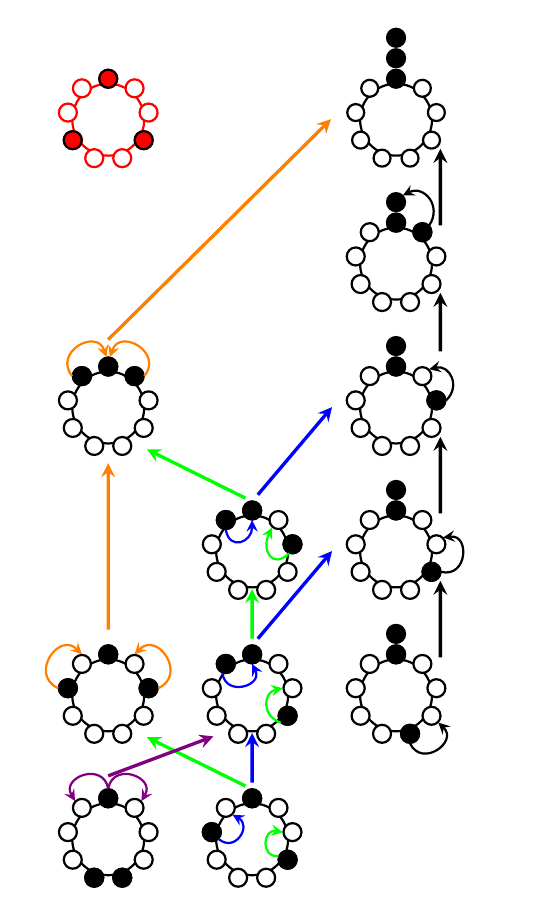
\begin{tikzpicture} [thick, node distance= 8em, >=stealth, ->, scale=0.65, transform shape, text centered] 
\node[rectangle, rounded corners=5pt](W) {};%{$-1, -1, 8$};
\node[right of = W, node distance=6em](test){};
\node[circle, minimum size =4em, draw, thick](CW){};
\foreach \i in {0, ..., 8}
\node[circle, minimum size =0.75em, draw, thick, fill=white]at(10- \i*40: 0.8)(W\i){};
\node[circle, minimum size =1em, draw, thick, fill=black]at(10-7*40: 0.8)(N1){};
\node[circle, minimum size =1em, draw, thick, fill=black]at(10-7*40: 1.2)(N2){};
\node[circle, minimum size =1em, draw, thick, fill=black]at(10-7*40: 1.6)(N3){};


\node[rectangle, rounded corners=5pt, below of =W](T0){};%{$-1, 0, 7$};
\node[circle, minimum size =4em, draw, thick, below of =W](CT0){};
\foreach \i in {0, ..., 8}
\node[circle, minimum size =1em, draw, thick, fill=white, below of =W\i](T0\i){};
\node[circle, minimum size =1em, draw, thick, fill=black, below of =N1](N1){};
\node[circle, minimum size =1em, draw, thick, fill=black, below of =N2](N2){};
\node[circle, minimum size =1em, draw, thick, fill=black, below of =W8](N3){};

\path (T08.north east) edge[bend right=75, looseness=1.5] (N2.north east);
\node[right of =T08, node distance= 1em](i10){};
\node[above of =i10, node distance = 5em](i01){};
\path (i10) edge[very thick] (i01);

\node[rectangle, rounded corners=5pt, below of = T0](T1){};%{$-1, 1, 6$};
\node[circle, minimum size =4em, draw, thick, below of =T0](CT1){};
\foreach \i in {0, ..., 8}
\node[circle, minimum size =1em, draw, thick, fill=white, below of =T0\i](T1\i){};
\node[circle, minimum size =1em, draw, thick, fill=black, below of =N1](N1){};
\node[circle, minimum size =1em, draw, thick, fill=black, below of =N2](N2){};
\node[circle, minimum size =1em, draw, thick, fill=black, below of =T00](N3){};

\path (T10.east) edge[bend right=75, looseness=1.5] (T18.north east);
\node[below of =i10, node distance= 7em](i21){};
\node[above of =i21, node distance = 4em](i12){};
\path (i21) edge[very thick] (i12);

\node[rectangle, rounded corners=5pt, below of = T1](T2){};%{$-1, 2, 5$};
\node[circle, minimum size =4em, draw, thick, below of =T1](CT1){};
\foreach \i in {0, ..., 8}
\node[circle, minimum size =1em, draw, thick, fill=white, below of =T1\i](T2\i){};
\node[circle, minimum size =1em, draw, thick, fill=black, below of =N1](N1){};
\node[circle, minimum size =1em, draw, thick, fill=black, below of =N2](N2){};
\node[circle, minimum size =1em, draw, thick, fill=black, below of =T11](N3){};

\path (T21.east) edge[bend right=100, looseness=2] (T20.north east);
\node[right of =T28, node distance= 1em](i32){};
\node[above of =i32, node distance = 5em](i23){};
\path (i32) edge[very thick] (i23);


\node[rectangle, rounded corners=5pt, below of = T2](T3){};%{$-1, 3, 4$};
\node[circle, minimum size =4em, draw, thick, below of =T2](CT1){};
\foreach \i in {0, ..., 8}
\node[circle, minimum size =1em, draw, thick, fill=white, below of =T2\i](T3\i){};
\node[circle, minimum size =1em, draw, thick, fill=black, below of =N1](N1){};
\node[circle, minimum size =1em, draw, thick, fill=black, below of =N2](N2){};
\node[circle, minimum size =1em, draw, thick, fill=black, below of =T22](N3){};

\path (T32.south) edge[bend right=100, looseness=2] (T31.south east);
\node[right of =T38, node distance= 1em](i43){};
\node[above of =i43, node distance = 5em](i34){};
\path (i43) edge[very thick] (i34);

\node[rectangle, rounded corners=5pt, left of = T2, node distance = 8 em](R1){};%{$0, 1, 5$};
\node[circle, minimum size =4em, draw, thick, left of =T2, node distance = 8 em](CR1){};
\foreach \i in {0, ..., 8}
\node[circle, minimum size =1em, draw, thick, fill=white, left of =T2\i, node distance = 8 em](R1\i){};
\node[circle, minimum size =1em, draw, thick, fill=black, left of =T27, node distance = 8 em](N1){};
\node[circle, minimum size =1em, draw, thick, fill=black, left of =T26, node distance = 8 em](N2){};
\node[circle, minimum size =1em, draw, thick, fill=black, left of =T20, node distance = 8 em](N3){};

\path (N2.south) edge[bend right=100, looseness=2, blue, in=-110] (N1.south);
\path (N3.250) edge[bend left=100, looseness=2, green, in=120] (R18.230);
\node[above of =N1, node distance= 0.5em](R1W){};
\node[left of =T15, node distance = 1em](T1R){};
\path (R1W) edge[blue, very thick] (T1R);

\node[rectangle, rounded corners=5pt, below of = R1](R2){};%{$0, 2, 4$};
\node[circle, minimum size =4em, draw, thick, below of = R1](CR2){};
\foreach \i in {0, ..., 8}
\node[circle, minimum size =1em, draw, thick, fill=white, below of =R1\i](R2\i){};
\node[circle, minimum size =1em, draw, thick, fill=black, below of =R17](N1){};
\node[circle, minimum size =1em, draw, thick, fill=black, below of =R16](N2){};
\node[circle, minimum size =1em, draw, thick, fill=black, below of =R11](N3){};

\path (N2.250) edge[bend right=100, looseness=2, blue] (N1.south);
\path (N3.south west) edge[bend left=75, looseness=1.5, green] (R20.west);
\node[above of =N1, node distance= 0.5em](R1W){};
\node[left of =T25, node distance = 1em](T2R){};
\node[below of =R17, node distance = 4em] (RR){};
\path (R1W) edge[blue, very thick] (T2R)
	 (R1W) edge[green, very thick] (RR);

\node[rectangle, rounded corners=5pt, below of = R2 ](R12){};%{$1, 2, 3$};
\node[circle, minimum size =4em, draw, thick, below of =R2 ](CR12){};
\foreach \i in {0, ..., 8}
\node[circle, minimum size =1em, draw, thick, fill=white,  below of =R2\i](R12\i){};
\node[circle, minimum size =1em, draw, thick, fill=black, below of =R27 ](N1){};
\node[circle, minimum size =1em, draw, thick, fill=black, below of =R25 ](N2){};
\node[circle, minimum size =1em, draw, thick, fill=black, below of =R21 ](N3){};

\path (N2.south east) edge[bend right=100, looseness=2, blue, in = -90 ] (R126.south east);
\path (N3.160) edge[bend left=100, looseness=2, green, in = 90] (R120.west);
\node[above of =N1, node distance= 0.5em](RtW){};
\node[below of =R27, node distance = 4em] (RR){};
\path (RtW) edge[blue, very thick] (RR);

\node[rectangle, rounded corners=5pt, left of = T1, node distance = 16em](S0){};%{$0, 0, 6$};
\node[circle, minimum size =4em, draw, thick, left of =T1, node distance= 16em](CS0){};
\foreach \i in {0, ..., 8}
\node[circle, minimum size =1em, draw, thick, fill=white, left of =T1\i, node distance= 16em](S0\i){};
\node[circle, minimum size =1em, draw, thick, fill=black, left of =T17, node distance= 16em ](N1){};
\node[circle, minimum size =1em, draw, thick, fill=black, left of =T16, node distance= 16em ](N2){};
\node[circle, minimum size =1em, draw, thick, fill=black, left of =T18, node distance= 16em ](N3){};

\path (N2.west) edge[bend left=100, looseness=2, orange] (N1.100);
\path (N3.east) edge[bend right=100, looseness=2, orange] (N1.80);
\node[above of =S07, node distance= 1.5em](S0T){};
\node[left of = W5, node distance = 1em](TS0){};
\path (S0T.center) edge[orange, very thick] (TS0);
\node[above of = R17, node distance = 0.5em](RS){};
\node[right of = S02, node distance = 1em](SR){};
\path (RS) edge[green, very thick] (SR);

\node[rectangle, rounded corners=5pt, below of = S0, node distance= 16em](S1){};%{$1, 1, 4$};
\node[circle, minimum size =4em, draw, thick, below of =S0, node distance= 16em](CS1){};
\foreach \i in {0, ..., 8}
\node[circle, minimum size =1em, draw, thick, fill=white, below of =S0\i, node distance= 16em](S1\i){};
\node[circle, minimum size =1em, draw, thick, fill=black, below of =S07, node distance= 16em](N1){};
\node[circle, minimum size =1em, draw, thick, fill=black, below of =S05, node distance= 16em](N2){};
\node[circle, minimum size =1em, draw, thick, fill=black, below of =S00, node distance= 16em](N3){};

\path (N2.west) edge[bend left=100, looseness=2, orange] (S16.north);
\path (N3.east) edge[bend right=100, looseness=2, orange] (S18.north);
\node[above of =S17, node distance= 1em](S1S0){};
\node[below of = S07, node distance = 5em](S0S1){};
\path (S1S0) edge[orange, very thick] (S0S1);
\node[right of =S12, node distance = 1em](SR){};
\path (RtW) edge[green, very thick] (SR);

\node[rectangle, rounded corners=5pt, below of = S1 ](R3){};%{$0, 3, 3$};
\node[circle, minimum size =4em, draw, thick, below of =S1 ](CR3){};
\foreach \i in {0, ..., 8}
\node[circle, minimum size =1em, draw, thick, fill=white, below of =S1\i ](R3\i){};
\node[circle, minimum size =1em, draw, thick, fill=black, below of =S17 ](N1){};
\node[circle, minimum size =1em, draw, thick, fill=black, below of =S13 ](N2){};
\node[circle, minimum size =1em, draw, thick, fill=black, below of =S12 ](N3){};

\path (N1.north) edge[bend right=100, looseness=2, violet] (R36.north west);
\path (N1.north) edge[bend left=100, looseness=2, violet] (R38.north east);
\node[above of =R37, node distance= 1.25em](S3Rter){};
\node[left of = R23, node distance = 1em](RterS3){};
\path (S3Rter.center) edge[violet, very thick] (RterS3);


\node[rectangle, rounded corners=5pt, above of = S0, red, node distance= 16em](S2){};%{$2, 2, 2$};
\node[circle, minimum size =4em, draw, thick, above of =S0, red, node distance= 16em](CS2){};
\foreach \i in {0, ..., 8}
\node[circle, red, minimum size =1em, draw, thick, fill=white, above of =S0\i, node distance= 16em](S2\i){};
\node[circle, minimum size =1em, draw, thick, fill=red, above of =S07, node distance= 16em](N1){};
\node[circle, minimum size =1em, draw, thick, fill=red, above of =S04, node distance= 16em](N2){};
\node[circle, minimum size =1em, draw, thick, fill=red, above of =S01, node distance= 16em](N3){};
\end{tikzpicture} 
}\hspace{0.2em}%%%%%%%%%%%%%%%%%%%%%%%%%%%%%%%%
\subfloat[) Strategies for 3 robots on a ring of 10 nodes.]{
\centering
\begin{tikzpicture} [thick, node distance= 8em, >=stealth, ->, scale=0.6, transform shape, text centered] 
\node[rectangle, rounded corners=5pt](W) {};%{$-1, -1, 8$};
\node[circle, minimum size =4em, draw, thick](CW){};
\foreach \i in {0, ..., 9}
\node[circle, minimum size =0.75em, draw, thick, fill=white]at(20- \i*36: 0.8)(W\i){};
\node[circle, minimum size =1em, draw, thick, fill=black]at(20-8*36: 0.8)(N1){};
\node[circle, minimum size =1em, draw, thick, fill=black]at(20-8*36: 1.2)(N2){};
\node[circle, minimum size =1em, draw, thick, fill=black]at(20-8*36: 1.6)(N3){};


\node[rectangle, rounded corners=5pt, below of =W](T0){};%{$-1, 0, 7$};
\node[circle, minimum size =4em, draw, thick, below of =W](CT0){};
\foreach \i in {0, ..., 9}
\node[circle, minimum size =1em, draw, thick, fill=white, below of =W\i](T0\i){};
\node[circle, minimum size =1em, draw, thick, fill=black, below of =N1](N1){};
\node[circle, minimum size =1em, draw, thick, fill=black, below of =N2](N2){};
\node[circle, minimum size =1em, draw, thick, fill=black, below of =W9](N3){};

\path (N3.north east) edge[bend right=75, looseness=1.5] (N2.north east);
\node[right of =T09, node distance= 1em](i10){};
\node[above of =i10, node distance = 5em](i01){};
\path (i10) edge[very thick] (i01);

\node[rectangle, rounded corners=5pt, below of = T0](T1){};%{$-1, 1, 6$};
\node[circle, minimum size =4em, draw, thick, below of =T0](CT1){};
\foreach \i in {0, ..., 9}
\node[circle, minimum size =1em, draw, thick, fill=white, below of =T0\i](T1\i){};
\node[circle, minimum size =1em, draw, thick, fill=black, below of =N1](N1){};
\node[circle, minimum size =1em, draw, thick, fill=black, below of =N2](N2){};
\node[circle, minimum size =1em, draw, thick, fill=black, below of =T00](N3){};

\path (T10.east) edge[bend right=75, looseness=1.5] (T19.north east);
\node[below of =i10, node distance= 7em](i21){};
\node[above of =i21, node distance = 4em](i12){};
\path (i21) edge[very thick] (i12);

\node[rectangle, rounded corners=5pt, below of = T1](T2){};%{$-1, 2, 5$};
\node[circle, minimum size =4em, draw, thick, below of =T1](CT1){};
\foreach \i in {0, ..., 9}
\node[circle, minimum size =1em, draw, thick, fill=white, below of =T1\i](T2\i){};
\node[circle, minimum size =1em, draw, thick, fill=black, below of =N1](N1){};
\node[circle, minimum size =1em, draw, thick, fill=black, below of =N2](N2){};
\node[circle, minimum size =1em, draw, thick, fill=black, below of =T11](N3){};

\path (T21.east) edge[bend right=100, looseness=2] (T20.north east);
\node[right of =T29, node distance= 1em](i32){};
\node[above of =i32, node distance = 5em](i23){};
\path (i32) edge[very thick] (i23);

\node[rectangle, rounded corners=5pt, below of = T2](T3){};%{$-1, 3, 4$};
\node[circle, minimum size =4em, draw, thick, below of =T2](CT2){};
\foreach \i in {0, ..., 9}
\node[circle, minimum size =1em, draw, thick, fill=white, below of =T2\i](T3\i){};
\node[circle, minimum size =1em, draw, thick, fill=black, below of =N1](N1){};
\node[circle, minimum size =1em, draw, thick, fill=black, below of =N2](N2){};
\node[circle, minimum size =1em, draw, thick, fill=black, below of =T22](N3){};

\path (T32.south east) edge[bend right=75, looseness=1.5] (T31.east);
\node[right of =T39, node distance= 1em](i43){};
\node[above of =i43, node distance = 5em](i34){};
\path (i43) edge[very thick] (i34);

\node[rectangle, rounded corners=5pt, below of = T3](T4){};%{$-1, 3, 4$};
\node[circle, minimum size =4em, draw, thick, below of =T3](CT4){};
\foreach \i in {0, ..., 9}
\node[circle, minimum size =1em, draw, thick, fill=white, below of =T3\i](T4\i){};
\node[circle, minimum size =1em, draw, thick, fill=black, below of =N1](N1){};
\node[circle, minimum size =1em, draw, thick, fill=black, below of =N2](N2){};
\node[circle, minimum size =1em, draw, thick, fill=black, below of =T33](N3){};

\path (T43.south) edge[gray, bend right=75, looseness=1.5] (T42.south east);
\path (T43.south) edge[gray, bend left=75, looseness=1.5] (T44.south west);
\node[right of =T49, node distance= 1em](i54){};
\node[above of =i54, node distance = 4.5em](i45){};
\path (i54) edge[gray, very thick] (i45);

\node[rectangle, rounded corners=5pt, left of = T2, node distance = 10 em](R1){};%{$0, 1, 5$};
\node[circle, minimum size =4em, draw, thick, left of =T2, node distance = 10 em](CR1){};
\foreach \i in {0, ..., 9}
\node[circle, minimum size =1em, draw, thick, fill=white, left of =T2\i, node distance = 10 em](R1\i){};
\node[circle, minimum size =1em, draw, thick, fill=black, left of =T28, node distance = 10 em](N1){};
\node[circle, minimum size =1em, draw, thick, fill=black, left of =T27, node distance = 10 em](N2){};
\node[circle, minimum size =1em, draw, thick, fill=black, left of =T20, node distance = 10 em](N3){};

\path (N2.south) edge[bend right=100, looseness=2, blue, in=-110] (N1.south);
\path (N3.250) edge[bend left=100, looseness=2, green, in=120] (R19.230);
\node[above of =N1, node distance= 0.5em](R1W){};
\node[left of =T16, node distance = 1em](T1R){};
\node[right of =S05, node distance = 1 em] (RS){};
\path (R1W) edge[blue, very thick] (T1R)
	 (R1W) edge[green, very thick] (RS);


\node[rectangle, rounded corners=5pt, below of = R1](R2){};%{$0, 2, 4$};
\node[circle, minimum size =4em, draw, thick, below of = R1](CR2){};
\foreach \i in {0, ..., 9}
\node[circle, minimum size =1em, draw, thick, fill=white, below of =R1\i](R2\i){};
\node[circle, minimum size =1em, draw, thick, fill=black, below of =R18](N1){};
\node[circle, minimum size =1em, draw, thick, fill=black, below of =R17](N2){};
\node[circle, minimum size =1em, draw, thick, fill=black, below of =R11](N3){};

\path (N2.250) edge[bend right=100, looseness=2, blue] (N1.south);
\path (N3.south west) edge[bend left=75, looseness=1.5, green] (R20.west);
\node[above of =N1, node distance= 0.5em](R1W){};
\node[left of =T26, node distance = 1em](T2R){};
\node[below of =R13, node distance = 0.5em] (RR){};
\path (R1W) edge[blue, very thick] (T2R)
	 (R1W) edge[green, very thick] (RR);

\node[rectangle, rounded corners=5pt, left of = T4, node distance = 7 em](Rbis){};%{$1, 2, 3$};
\node[circle, minimum size =4em, draw, thick, left of =T4, node distance = 7 em](CR12){};
\foreach \i in {0, ..., 9}
\node[circle, minimum size =1em, draw, thick, fill=white,  left of =T4\i, node distance = 7 em](Rbis\i){};
\node[circle, minimum size =1em, draw, thick, fill=black, left of =T48, node distance = 7 em](N1){};
\node[circle, minimum size =1em, draw, thick, fill=black, left of =T47, node distance = 7 em](N2){};
\node[circle, minimum size =1em, draw, thick, fill=black, left of =T42, node distance = 7 em](N3){};

\path (N2.250) edge[bend right=100, looseness=2, blue] (N1.south);
\path (N3.north west) edge[bend left=100, looseness=2, green] (Rbis1.north west);
\node[above of =N1, node distance= 0.5em](RbW){};
\node[left of =T34, node distance = 1em](T3R){};
\node[below of =R23, node distance = 0.5em] (RR){};
\path (RbW) edge[blue, very thick] (T3R)
	 (RbW) edge[green, very thick] (RR);

\node[rectangle, rounded corners=5pt, left of = Rbis, node distance = 6 em](Rter){};%{$1, 2, 3$};
\node[circle, minimum size =4em, draw, thick, left of =Rbis, node distance = 6 em](CR12){};
\foreach \i in {0, ..., 9}
\node[circle, minimum size =1em, draw, thick, fill=white, left of =Rbis\i, node distance = 6 em ](Rter\i){};
\node[circle, minimum size =1em, draw, thick, fill=black, left of =Rbis8, node distance = 6 em ](N1){};
\node[circle, minimum size =1em, draw, thick, fill=black, left of =Rbis6, node distance = 6 em ](N2){};
\node[circle, minimum size =1em, draw, thick, fill=black, left of =Rbis1, node distance = 6 em ](N3){};

\path (N2.south east) edge[bend right=100, looseness=2, blue, in = -90 ] (Rter7.south east);
\path (N3.west) edge[bend left=100, looseness=2, green, in = 90] (Rter0.west);
\node[above of =N1, node distance= 0.5em](RtW){};
\node[below of =R23, node distance = 0.5em] (RR){};
\path (RtW) edge[blue, very thick] (RR);

\node[rectangle, rounded corners=5pt, left of = T1, node distance = 20em](S0){};%{$0, 0, 6$};
\node[circle, minimum size =4em, draw, thick, left of =T1, node distance= 20em](CS0){};
\foreach \i in {0, ..., 9}
\node[circle, minimum size =1em, draw, thick, fill=white, left of =T1\i, node distance= 20em](S0\i){};
\node[circle, minimum size =1em, draw, thick, fill=black, left of =T17, node distance= 20em ](N1){};
\node[circle, minimum size =1em, draw, thick, fill=black, left of =T18, node distance= 20em ](N2){};
\node[circle, minimum size =1em, draw, thick, fill=black, left of =T19, node distance= 20em ](N3){};

\path (N1.west) edge[bend left=100, looseness=2, orange] (N2.100);
\path (N3.east) edge[bend right=100, looseness=2, orange] (N2.80);
\node[above of =S08, node distance= 1.5em](S0T){};
\node[left of = W5, node distance = 1em](TS0){};
\path (S0T.center) edge[orange, very thick] (TS0);

\node[rectangle, rounded corners=5pt, below of = S0, node distance = 16em](S1){};%{$1, 1, 4$};
\node[circle, minimum size =4em, draw, thick, below of =S0, node distance = 16em](CS1){};
\foreach \i in {0, ..., 9}
\node[circle, minimum size =1em, draw, thick, fill=white, below of =S0\i, node distance = 16em](S1\i){};
\node[circle, minimum size =1em, draw, thick, fill=black, below of =S08, node distance = 16em](N1){};
\node[circle, minimum size =1em, draw, thick, fill=black, below of =S06, node distance = 16em](N2){};
\node[circle, minimum size =1em, draw, thick, fill=black, below of =S00, node distance = 16em](N3){};

\path (N2.west) edge[bend left=100, looseness=2, orange] (S17.north);
\path (N3.east) edge[bend right=100, looseness=2, orange] (S19.north);
\node[above of =S18, node distance= 1em](S1S0){};
\node[below of = S03, node distance = 1em](S0S1){};
\path (S1S0) edge[orange, very thick] (S0S1);
\node[right of =S12, node distance = 1em](SR){};
\path (RtW) edge[green, very thick] (SR);
 
\node[rectangle, rounded corners=5pt, below of = S1, node distance = 16em](S2){};%{$2, 2, 2$};
\node[circle, minimum size =4em, draw, thick, below of =S1, node distance = 16em](CS2){};
\foreach \i in {0, ..., 9}
\node[circle, minimum size =1em, draw, thick, fill=white, below of =S1\i, node distance = 16em](S2\i){};
\node[circle, minimum size =1em, draw, thick, fill=black, below of =S18, node distance = 16em](N1){};
\node[circle, minimum size =1em, draw, thick, fill=black, below of =S15, node distance = 16em](N2){};
\node[circle, minimum size =1em, draw, thick, fill=black, below of =S11, node distance = 16em](N3){};

\path (N2.west) edge[bend left=100, looseness=2, orange] (S26.north);
\path (N3.east) edge[bend right=100, looseness=2, orange] (S20.north);
\node[above of =S28, node distance= 1em](S2S1){};
\node[below of = S13, node distance = 1em](S1S2){};
\path (S2S1) edge[orange, very thick] (S1S2);

\node[rectangle, rounded corners=5pt, right of = S2, node distance = 10 em](SS3){};%{$0, 3, 3$};
\node[circle, minimum size =4em, draw, thick, right of =S2, node distance = 10 em](CSS3){};
\foreach \i in {0, ..., 9}
\node[circle, minimum size =1em, draw, thick, fill=white, right of =S2\i, node distance = 10 em](SS3\i){};
\node[circle, minimum size =1em, draw, thick, fill=black, right of =S28, node distance = 10 em](N1){};
\node[circle, minimum size =1em, draw, thick, fill=black, right of =S24, node distance = 10 em](N2){};
\node[circle, minimum size =1em, draw, thick, fill=black, right of =S22, node distance = 10 em](N3){};

\path (N1.north) edge[bend right=100, looseness=2, violet] (SS37.north west);
\path (N1.north) edge[bend left=100, looseness=2, violet] (SS39.north east);
\node[above of =SS38, node distance= 1.25em](S3Rter){};
\node[below of = Rter3, node distance = 0.5em](RterS3){};
\path (S3Rter.center) edge[violet, very thick] (RterS3);

\end{tikzpicture}
}
\caption{Strategies from Uppaal Tiga.} 
\label{fig:Strat}
\end{figure}
The red configuration is the configuration from which there is no strategy since it is periodical.
For each other configuration, the actions chosen by the strategy are depicted by small arrows on the ring, 
path on the graph show the result of these actions in a synchronous execution model (it represents the adversary actions).
Paths and actions are colored in order to distinguish the different types of configurations:  
The black ones are for the tower configurations without symmetries, grey ones for 
tower configurations with an axe of symmetry.
The orange ones depict the symmetrical configurations:  $\equivclass{\{(f_1, f_1, f_2), (f_2, f_1, f_1)\}}$ with $-1 < f_1 < f_2$, 
the symmetrical configurations:  $\equivclass{\{(f_1, f_1, f_2), (f_2, f_1, f_1)\}}$ with $-1 < f_2 < f_1$ are the violet ones.
The blue and green ones depict the two different strategies from rigid configurations.

From the given strategies we extract a pattern and thus a parameterized strategy:  
\begin{itemize}%[parsep=0cm, itemsep=0cm, topsep=0cm] 
	\item If $2$ robots form a tower the last robot takes the shortest path to the tower:  
		\begin{itemize}
		\item From $\equivclass{\{(-1, \frac{n}{2}-1, \frac{n}{2}-1), (\frac{n}{2}-1, \frac{n}{2}-1, -1)\}}$ the edge relation leads to 
		$(\{(-1, \frac{n}{2}-1, \frac{n}{2}-1), (\frac{n}{2}-1, \frac{n}{2}-1, -1)\}, (\still, \still, \disoriented))$.
		\item From $\equivclass{\{(-1, f_1, f_2), (f_2, f_1, -1)\}}$ when $f_1 \neq \frac{n}{2}-1$ the edge relation leads to 
		$(\{(-1, f_1, f_2), (f_2, f_1, -1)\}$with $-1< f_1 < f_2, (\still, \still, \counterclockwise))$.
		\end{itemize}
	\item If the configuration is symmetrical, in$\equivclass{\{(f_1, f_1, f_2), (f_2, f_1, f_1)\}}$ 
	with $-1 < f_1$, $-1 < f_2$, and $f_1 \neq f_2$, 
	the proposed strategy depends on whether $f_1 < f_2$ or $f_2 < f_1$:  
	\begin{itemize}%[parsep=0cm, itemsep=0cm, topsep=0cm] 	
		\item  If $f_1 < f_2$ then the two symmetrical robots get closer to the last robot.  %[$r_{s1}$]
		The edge relation leads to $((f_1, f_1, f_2), (\clockwise, \still, \counterclockwise))$.
		\item  If $f_1 > f_2$ then the disoriented robot moves. %[$r_{s2}$] 
		The edge relation leads to $((f_2, f_1, f_1), (\still, \still, \disoriented))$.
	\end{itemize}
	\item If the configuration is rigid ($\equivclass{\{(f_1, f_2, f_3), (f_3, f_2, f_1)\}}$ with $-1< f_1< f_2<f_3$) 
	there are three possible algorithms:  
	\begin{itemize}%[parsep=0cm, itemsep=0cm, topsep=0cm] 
		\item The robot with the minimum view gets closer to its nearest neighbor. %24  [$r_{24}$] 
	In this case the edge relation leads to $(\{(f_1, f_2, f_3), (f_3, f_2, f_1)\}, (\clockwise, \still, \still))$.
		\item The robot with the maximum view gets closer to its nearest neighbor. %17 [$r_{17}$]
	 In this case the edge relation leads to $(\{(f_1, f_2, f_3), (f_3, f_2, f_1)\}, (\still, \still, \counterclockwise))$.
		\item The robot with the minimum view and the robot with the maximum view get
		closer to their nearest neighbor.
	In this case the edge relation leads to $(\{(f_1, f_2, f_3), (f_3, f_2, f_1)\}, $ $(\clockwise, \still, \counterclockwise))$.
		This strategy is the two above strategies made simultaneously.%15[$r_{r15}$]
	\end{itemize}
%	Thus, the edge relation for rigid configuration leads to:  $\{((f_1,   f_2, f_3), (a_1, \still, a_2))\}$, 
%	with $a_1\in \{\clockwise, \still\}$, $a_2 \in \{\still, \counterclockwise\}$ and $a_1 \neq a_2$.
\end{itemize}

From Theorem~\ref{th: correctness}, one can translate the winning strategies for each configuration
into a distributed algorithm.
We present the possible strategies in Table~\ref{tab: algoSynth}.
For robot views not present in the Table, the robot movement is $\Idle$. 
The strategies are correct by construction. They have been obtained with various values of $n$ as input ($3 \leq n  \leq 15$, $n = 100$). 

\begin{table*}[htbp]
\centering
\begin{tabular}{|c l c l c l|}
\hline
\multicolumn{6}{|l|}{\rule[0.1cm]{0cm}{0.25cm}  
\textbf{3-gathering algorithm:  }}
\\[1pt] \hline
Rule: :  & Condition & $\land$ & $\view(r, c)$&$\rightarrow$&Move\\
\hline
$\textcolor{gray}{RS1}$: : & & &$(R_1, F_{\frac{n}{2}-1}, T_2, F_{\frac{n}{2}-1})$&$\rightarrow$&$r.\Doubt$\\
$RS2$: : & $f_1 \neq f_2$&$\wedge $&$(R_1, F_{f_1}, T_2, F_{f_2})$&$\rightarrow$&$r.\?$\\
$\textcolor{orange}{RS3}$: : & $-1< f_1 < f_2$&$\wedge $&$(R_1, F_{f_1}, R_1, F_{f_1}, R_1, F_{f_2})$&$\rightarrow$&$r.\Front$\\
$\textcolor{violet}{RS4}$: : & $-1< f_2 < f_1$&$\wedge $&$(R_1, F_{f_1}, R_1, F_{f_2}, R_1, F_{f_1})$&$\rightarrow$&$r.\?$\\
$\textcolor{blue}{RS5_1}$: : &$-1< f_1< f_2<f_3$&$\wedge $&$(R_1, F_{f_1}, R_1, F_{f_2}, R_1, F_{f_3})$&$\rightarrow$&$r.\Front$\\
$\textcolor{green}{RS5_2}$: : &$-1< f_1< f_2<f_3$&$\wedge $&$(R_1, F_{f_2}, R_1, F_{f_1}, R_1, F_{f_3})$&$\rightarrow$&$r.\Front$\\
\hline
\end{tabular}
\caption{Rules of the synthesized algorithm for a robot $r$}
\label{tab: algoSynth}
\end{table*}



\subsection{Proof of the 3-gathering algorithm}
\label{preuve2}
Let $C=\equivclass{\{(x,y,z),(z,y,x)\}}$ be a class of configurations such that $\rep(C)= (\{x,y,z),(z,y,x)\})$ when $x \leq y \leq z$, and $d=x+y$ be the \emph{separating-distance} of $C$.


	\begin{theorem}
Starting from any configuration (except periodic ones) the 3-gathering algorithm %\ref{alg: genstrat} 
eventually reaches a gathering configuration.
\end{theorem}

\begin{proof} 
The theorem is correct if each of the movements produced by the above strategy %\ref{alg: genstrat} 
is decreasing the separating-distance.
The proof directly follows from the Lemmas \ref{lemma: tower}, \ref{lemma: rigid}, \ref{lemma: sym1}, \ref{lemma: sym2} below. 
Each one of these lemmas addresses a possible initial class of configurations and yields a stronger result.
\end{proof}

\begin{lemma}
\label{lemma: tower}
Starting from a class of configurations $\equivclass{(-1, d_2, d_3)}$, %such that $\rep(\equivclass{(-1, d_2, d_3)}) =  (-1, d_2, d_3)$, 
which is the class of configurations where there is one tower of size 2, the system executing  the 3-gathering algorithm %\ref{alg: genstrat} 
 eventually reaches a gathering configuration. 
\end{lemma}

	\begin{proof}\hfill
	\begin{description}%[parsep=0cm, itemsep=0cm, topsep=0cm]
		\item [Base-case:  ] Consider the minimal separating distance. For any ring size $n \in \mathbb{N}$, the execution starting from
	 		$\equivclass{\{(-1, 0, n-2),(n-2,0,-1)\}}$ leads to $\equivclass{\{(-1, -1, n-1),(n-1,-1,-1)\}}$ which is 
			the gathering class of configuration.
		 \item [Induction:  ] Assume that starting in a configuration where the separating-distance
			is $i \in \mathbb{N}$, the system executing the strategy %\ref{alg: genstrat}
			eventually reaches a gathering  class of configuration. We prove in the following that the above
			also holds	 when the \emph{separating-distance} is $i+1$:  \\
			From $\equivclass{\{(-1, i+2, d_3),(d_3,i+2,-1)\}}$ the execution of the strategy leads 
			to $\equivclass{\{(-1, i+1, d_3+1),(d_3+1,i+1,-1)\}}$.
			The proof follows from the induction hypothesis. 
	\end{description}
	\end{proof}
	
\begin{lemma}
\label{lemma: rigid} %refaire sasn regle avec any of the rules ...
\label{lemma: rigid15}
Starting from a rigid configuration $\equivclass{\{(d_1, d_2, d_3),(d_3,d_2,d_1)\}}$, the system executing  the $3$-gathering algorithm %\ref{alg: genstrat}
eventually reaches a gathering configuration.
\end{lemma}

From a rigid configuration $\equivclass{\{(d_1, d_2, d_3),(d_3,d_2,d_1)\}}$ where 
%$\rep(\equivclass{\{(d_1, d_2, d_3),(d_3,d_2,d_1)\}}) = $ 
the representative is $\{(d_1, d_2, d_3),(d_3,d_2,d_1)\}$, with $-1 < d_1 < d_2 < d_3$, 
the algorithm reaches a gathering configuration.
In order to prove this lemma for the last edge we fix $d_1=0$
and prove that for any $d_2$ and any $d_3$ the strategy is correct, 
and then we use this proof as a base case to prove the lemma
for any $d_1, d_2$ and $d_3$.
	
	\begin{proof}\hfill
	%15
	\begin{description}%[parsep=0cm, itemsep=0cm, topsep=0cm]
		\item [Base-case2:  ] 
	When $d_1=0$, for any $d_2, d_3$, from $\equivclass{\{(0, d_2, d_3),(d_3,d_2,0)\}}$ the strategy 
	leads to $\equivclass{\{(-1, d_2-1, d_3+2),(d_3+2,d_2-1,-1)\}}$ where the \emph{separating-distance} is decreased by two.
	Hence, the lemma is true, thanks to lemma~\ref{lemma: tower}.
		 \item [Induction2:  ]%sur y  
	We assume that the gathering is made for any $d_2, d_3$ for 
	an $d_1=i$, and we show that it is also made when $d_1=i+1$.
	From $\equivclass{\{(i+1, d_2, d_3),(d_3,d_2,i+1)\}}$ the algorithm leads to $\equivclass{\{(i-1, d_2-1, d_3+2),(d_3+2,d_2-1,i-1)\}}$.
	The separating distance is decreased.
	Thanks to our induction hypothesis and Lemma \ref{lemma: tower} (for the tower case) the lemma is true. 
	\end{description}
	\end{proof}


\begin{lemma}
\label{lemma: sym1}
Starting from a symmetrical class of configurations $(\equivclass{\{(d_1, d_1, d_2),(d_2,d_1,d_1)\}})$ without tower where 
$\rep(\equivclass{\{(d_1, d_1, d_2),(d_2,d_1,d_1)\}}) =  \{(d_1, d_1, d_2),(d_2,d_1,d_1)\}$, with $-1 < d_1$, $-1 < d_2$, and $d_1 \neq d_2$.
The 3-gathering algorithm %\ref{alg: genstrat}  
eventually reaches a gathering configuration.
\end{lemma}
	
	\begin{proof}\hfill	%Cas 1 2 
	\begin{description}%[parsep=0cm, itemsep=0cm, topsep=0cm]
		\item [Base-case:  ] 
			Consider the class of configurations where the \emph{separating-distance} is minimal:  $\equivclass{\{(0, 0, n-3),(n-3,0,0)\}}$. 
			For any ring size $n \in \mathbb{N}$, the system executing the 3-gathering algorithm starting in 
			$\equivclass{\{(0, 0, n-3),(n-3,0,0)\}}$ reaches 
			$\equivclass{\{(-1, -1, n-1),(n-1,-1,-1)\}}$ (the gathering class of configurations). 
		 \item [Induction:  ] 
			Assume that when the separating-distance equals $2i, i \in \mathbb{N}$ a gathering configuration is eventually
			reached, and prove that it is also true when the separating distance is $2i+2$.
			From $\equivclass{\{(i+1, i+1, d_3),(d_3,i+1,i+1)\}}$ the system executing the strategy %\ref{alg: genstrat} 
			eventually reaches $\equivclass{\{(i, i, d_3+2),(d_3+2,i,i)\}}$.
	 		The lemma follows from the induction hypothesis. 
	\end{description}
	\end{proof}
	
\begin{lemma}
\label{lemma: sym2}
Starting from a symmetrical class of configurations $\equivclass{\{(d_1, d_1, d_2),(d_2,d_1,d_1)\}}$ without tower where 
$\rep(\equivclass{\{(d_1, d_1, d_2),(d_2,d_1,d_1)\}}) =  \{(d_2, d_1, d_1),(d_2,d_1,d_1)\}$, with $-1 < d_1$, $-1 < d_2$, and $d_1 \neq d_2$.
The 3-gathering algorithm eventually reaches a gathering configuration.
\end{lemma}
	
	\begin{proof}
	First observe that $\equivclass{\{(d_1, d_1, d_2),(d_2,d_1,d_1)\}}$ leads to $\equivclass{\{(d_1-1, d_1+1, d_2),(d_2,d_1+1,d_1-1)\}}$.
	The obtained configuration is a symmetric configuration if $d_2=d_1-1$
	or a rigid configuration otherwise. Thanks to Lemma~\ref{lemma: sym1} and Lemma~\ref{lemma: rigid15}, we know that from these configurations, a gathering configuration is eventually reached.
	\end{proof}  


%\subsection{Conclusion}

We proposed a formal method based on reachability games that permits to automatically generate distributed algorithms for mobile autonomous robots solving a global task. The task of gathering on a ring-shaped network was used as a case study. We hereby discuss current limitations and future works.

While our construction generates algorithms for a particular number of robots $k$ and ring size $n$, the game encoding we propose enables to easily tackle the gathering problem for any given $k$ and $n$, provided as inputs, since $k$ and $n$ are parameters of the arena. Also, we focused on the atomic Fsync and Ssync models. Breaking the atomicity of Look-Compute-Move cycles (that is, considering automatic algorithm production for the Async model) implies that robots cannot maintain a current global view of the system (their own view may be outdated), nor be aware of the view of other robots (that may be outdated as well). Then, our two-players game encoding is not feasible anymore. A natural approach would be to use distributed games, but they are generally undecidable as previously stated. So, a completely new approach is required for the automatic generation of non-atomic mobile robot algorithms.


%%%%%%%%%%%%%%%%%%%%%%%%%%%%%%%%%%%%%%%%%%%%%%%%%%%%%%%%%%%%%%%%%%%%%%%%
%%%%%%%%%%%%%%%%%%%%%%%%%%%%%%%%      Async     %%%%%%%%%%%%%%%%%%%%%%%%%%%%%%%%%
%%%%%%%%%%%%%%%%%%%%%%%%%%%%%%%%%%%%%%%%%%%%%%%%%%%%%%%%%%%%%%%%%%%%%%%%
		

	
\chapter[Asynchronous Synthesis]{Synthesis of asynchronous mobile robot protocols}
\label{chap:asynth}
In this chapter we consider the asynchronous model. 
We first show how finding an algorithm for gathering asynchronous robots 
can be seen as a two-player game with partial information. In contrast, the game 
considered in the previous chapter was a \emph{perfect information} game.
In order to fight the combinatorial explosion due to the asynchronous model
we propose a recursive algorithm that permits to obtain a gathering
protocol in the asynchronous model thanks to synchronous 
synthesis and model checking. 	

Recall that in the asynchronous model, some robots can be in a computation state while others are in a moving state, 
leading to the possibility for a robot to  move according to an obsolete observation. Therefore, the game must be modified 
from the synchronous case:  We show in the sequel how this new setting corresponds to a 
\emph{partial observation game}.





\section {Partial observation games}	\index{two-player games with partial observation}	
%has perfect information if each player, when making any decision, is perfectly informed of all the events that have previously occurred
Games can be classified according to the knowledge of the players about the game:  
In a partial observation game, the set of locations is partitioned into sets called observations. 
A player cannot see the current location of the game, but only its observation.
For example, in the asynchronous model, a robot cannot see the states of other robots.
There are three types of games according to observations:  
 complete-observation games, where both players have complete knowledge of the game
(as was the case of the game in the previous section), partial-observation games, where 
each player only has a partial view about the state 
and the moves of the other player, and one-sided partial-observation games, where one player has partial knowledge 
and the other one has complete knowledge of the game.
 
 Two-player games with partial observations are considerably more complicated than games with complete observations.
 Decision problems for partial observation games usually lie in higher complexity classes than 
complete-observation games~\cite{Reif1984274}.
%\todo{chatterjee doyen:  decidability ... undecidability ...}


\bigskip
In this section we recall classical notions (from~\cite{doyen+raskin}). 
A partial observation game is composed of an \emph{arena} and \emph{winning conditions}.

An arena for a game with partial observation is a graph $\arena = ( V, E, O)$ in which the set of vertices
$V=V_p\uplus V_a$ is partitioned into $V_p$, the player locations, and $V_a$
the adversary locations.  
The set of edges is $E\subseteq V\times V$, 
and $O \subseteq 2^{V}$ is a finite set of observations that partitions the set  $V$ of vertices. 
It induces a mapping $\mathcal{O}:  V \to O$ that associates with each vertex its unique observation.
For each play $\pi = v_0v_1\dots$ in $V^\infty$, we denote by $\mathcal{O}(\pi)$ the sequence $\mathcal{O}(v_0)\mathcal{O}(v_1)\dots$, 
we analogously extend observations to histories, sets of plays, etc.

A game is played in the same way as in the perfect information case, but now only the observation 
of the current location is revealed to the player who owns the location. The effect of uncertainty 
about the history of the play is formally captured by the notion of observation-based strategy.
An observation-based strategy for the player is a function $\sigma^\mathcal{O}:  V^*\cdot V_p \rightarrow V$ 
such that $\sigma^\mathcal{O}(\pi) = \sigma^\mathcal{O}(\pi')$ for all histories $\pi, \pi' $ in $V^*\cdot V_p$ with 
$\mathcal{O}(\pi) = \mathcal{O}(\pi')$.

\begin{example}
In the game with partial observation depicted in Figure~\ref{fig:partSynth}
player vertices are represented by rectangles and adversary positions by circles.
The observations of the player are $O1 = \{P1, P2\}$, $O2 = \{P3, P4\}$. 
The transitions are shown as labeled edges, and the initial state is $\textit{Init}$. 
The objective of the player is $\Reach(T)$. 
This game is not winning for the player.
If the strategy is to take the action $a$ in $O1$ it is only winning in $P2$, and if the strategy is 
to take the action $b$ in $O1$, it is only winning in $P1$.
\begin{figure}[h]
\centering
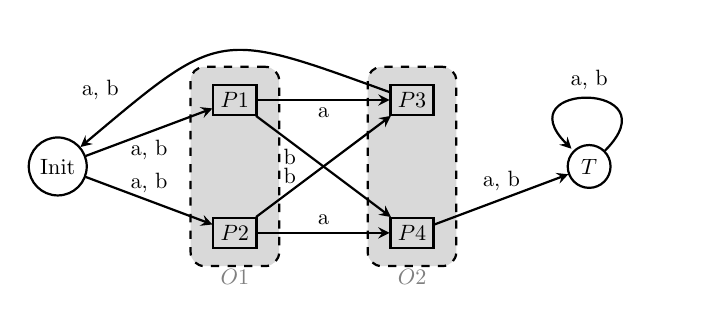
\begin{tikzpicture} [thick, node distance= 8em, >=stealth, ->, scale=0.8, transform shape] 
\node[circle, draw, text centered](A1){Init};
\node[right of = A1](A2){};
\node[rectangle, rounded corners=5pt, draw, dashed, fill = gray!30, right of =A1, minimum width = 4em, minimum height = 9em]($O1$){};
\node[rectangle, draw, text centered, above of = A2, node distance = 3em](P1) {$P1$};
\node[rectangle, draw, text centered, below of = A2, node distance = 3em](P2) {$P2$};
\node[below of = P2, node distance = 2em](o1){\textcolor{gray}{$O1$}};
\node[right of = A2](A3){};
\node[rectangle, rounded corners=5pt, draw, dashed, fill = gray!30, right of =A2, minimum width = 4em, minimum height = 9em]($O2$){};
\node[rectangle, draw, text centered, above of = A3, node distance = 3em](P3) {$P3$};
\node[rectangle, draw, text centered, below of = A3, node distance = 3em](P4) {$P4$};
\node[below of = P4, node distance = 2em](o2){\textcolor{gray}{$O2$}};
\node[circle, draw, text centered, right of = A3](T){$T$};
\path (A1) edge[] node[below, text centered]{a, b} (P1) 
         	edge[] node[above, text centered]{a, b}(P2)
	(P2) edge[] node[above, text centered]{a}(P4) 
		edge[] node[above, near start]{b}(P3)
	(P1) edge[] node[below, near start]{b} (P4) 
		edge[]node[below]{a} (P3)
	(P3) edge[bend right, looseness = 1.5]node[above left, very near end]{a, b} (A1)
	(P4) edge[]node[above, text centered]{a, b} (T)
	(T) edge[loop]node[above, text centered]{a, b} (T);
	
\end{tikzpicture} 
\caption{A partial observation game with a reachability objective} 
\label{fig:partSynth}
\end{figure}
\end{example}


\section{The arena for asynchronous robots}
\label{sub sub:arenaAsync}
We now explain how a gathering algorithm for the robots in the asynchronous model can be obtained 
as a winning strategy in a one-sided partial observation game. Like before, the adversary is the scheduler that can dynamically 
decide robot chirality at every activation, with complete observation. In order to take into account asynchronous moves of robots 
in the scheduling, the vertices of the associated arena must now contain robot states and planned move of robots that are not yet scheduled 
(and can thus become obsolete).  On the other hand, the player is the algorithm deciding robot moves in every state.
Since robot execution of a rule is only based on its view, the player has a partial observation of the location.

Robot states are described by tuples in $S=\{\Front, \Back, \Idle, \RLC \}^k$, 
where $\RLC$ denotes the ``Ready to Look-Compute'' state (see Figure~\ref{fig:ring}). 
For the implementation, all robot movements must relate to ring positions. 
 We consider the arena $\arena=(V_p\uplus V_a, E, O)$, where:  
 \begin{itemize}
 \item The set of player vertices is $V_p= (\ObsClass \times \Past)$; 
  \item The set of adversary vertices is $V_a= \Obs \times \Past \times \Actions^k$; 
 \item  As in the synchronous arena the edge relation ensures a strict alternation between
 the two players:  $E\subseteq (V_p\times V_a) \cup (V_a\times V_p)$;
 \item The observation simply abstracts away the robot states, hence $O= \ObsClass$ and 
 the mapping $\mathcal{O}$ is only defined for player vertices by $\mathcal{O}(v) = \obs$ for 
 $v= (\obs, \mem ) \in V_p$.
 \end{itemize}
 
These elements are detailed in the sequel.
 
\subsection{Edges from $V_p$ to $V_a$}

A player vertex $v= (\obs, \mem) \in V_p$ is built as follows. We consider the canonical configuration $c_o$ 
associated with $o=\rep(\obs)$, defined by $c_o(r_1)=0$, $c_o(r_2)=f_1+1, \dots, c_o(r_k) = \Sigma_{i=1}^k f_i \plusN k$, 
where robot $r_i$ is at distance $f_i$ of robot $r_{i \plusK 1}$, and $s=(s_1, \ldots, s_k)$ where $s_i$ is the state of $r_i$.

The player chooses robot movements by applying some decision function related to the views of the 
equivalence class $\mathcal{O}(v)=\obs$, similarly to the synchronous case:  
There is an edge $(v, v')$ in $E$ with $v'=\bigl (o, \mem, (a_1, \dots, a_k)\bigr )$ if and only if there exists 
a decision function $\partial$ such that $a_i=\dec(\view(r_i, c_o))$ for all $i$ in  $[1.. k]$.  

The play continues on an adversary position memorizing the different movements
decided for each robot.
Note that at this step the player chooses the strategy: he does not choose the robot effective movement.


\subsection{Edges from $V_a$ to $V_p$}
From a position $v= \bigl (o, \mem, (a_1, \dots, a_k)\bigr ) \in V_a$, the adversary 
chooses a set $\Sched \subseteq \Rob$ of robots, and schedules them to act according to their 
current state $\mem$.
When disoriented robots are scheduled for their $\LC$ actions the adversary also 
chooses the direction in which robots will move, producing  
the next player vertex of the form $(\obs', \mem' ) \in V_p$ .

To  describe the edge more precisely, given a set $\Sched$ and $v \in V_a$, we define the 
corresponding $(v, \Sched)$-move and the $(v, \Sched)$-consistent states, in the vein of $v$-consistent 
movements of Definition~\ref{def:vCo} in Chapter~\ref{chap:synth}.

The $(v, \Sched)$-move $m$ is the unique movement associated 
 with $v$ when subset $\Sched$ of robots is scheduled. 
 \begin{definition}\label{def:mCo}
 For a state $v= \bigl (o, \mem, (a_1, \dots, a_k)\bigr ) \in V_a$ and a set of robots
 $\Sched \subseteq \Rob$,  the $(v, \Sched)$-move 
 $m = (m_1, \dots, m_k)\in(\Actions \cup   \{-\} \setminus \{\?\})^k$ is defined
for all $1 \leq i \leq k$ by: \\ $$m_i= \begin{cases}
 s_i & \textit{if } r_i \in \Sched \textit{ and } s_i \neq \RLC \\
 - &\textit{otherwise}
 \end{cases}$$
 \end{definition}
The $-$ represents an absence of movement for a robot, corresponding to the robot 
 being either not scheduled or in its $\RLC$ state (see Definition~\ref{def:prod}).
 Note that movements in $m$ have been determined on some previous adversary position.

A $(v, \Sched)$-consistent state $s'$ represents the scheduler choices in term of direction for disoriented robots, 
resolving $\?$ moves.
When a robot is not scheduled its state stays the same. 
If the robot is scheduled, its new state depends on its current state:  if the robot state is in either $\Front$ or $\Back$ then 
it actually performs the move (we have $m_i = \mem_i$) and its state becomes $\RLC$. If the robot state is $\RLC$ then 
its new state is $a_i$ if $a_i \neq \Doubt$, and otherwise the scheduler chooses among $\Front$ or $\Back$. 
\begin{definition}\label{def:mapCo}
 For a vertex $v= \bigl (o, \mem, (a_1, \dots, a_k)\bigr ) \in V_a$ and a set 
 $\Sched \subseteq \Rob$ of robots, a $(v, \Sched)$-consistent state $\mem' =(s'_1, \ldots, s'_k) \in \Past$ is defined 
 for all $1 \leq i \leq k$
 by:  \begin{itemize}
 \item if $r_i \notin \Sched$,  then $s'_i =  s_i$, 
 \item if $r_i \in \Sched$ and $s_i \neq \RLC$,  then $s'_i =   \RLC$, 
 %$s'_i = a_i$
 \item if $r_i \in \Sched$, $s_i = \RLC$ and  $a_i \neq \Doubt$,  then there are two cases, 
	 \begin{itemize}
	\item If $\view^{\min\_r_i} \circlearrowright ^m \view^{\min\_r_0}$ for some $m$ then
		$s'_i = a_i$.
	\item Otherwise $s'_i = \overline{a_i}$. 
	\end{itemize}
	(We choose the direction sense of  $\view^{\min\_r_0}$  as the common sense of direction.)
 \item otherwise $s'_i \in \{\Front, \Back\}$.
 \end{itemize}
 Note that the last case corresponds to $r_i \in \Sched$, $s_i = \RLC$ and $a_i = \Doubt$.
 \end{definition}
 
 
%oplus definition
The effect on an observation, of any movement $m_i$ of robot $r_i$ can be described by a mapping 
$\varepsilon:  \{1, \dots, k\}\times\{\Front, \Back, \Idle\} \to \{-1, 0, 1\}^k$.
This mapping denotes the translated moves that permit to apply real movements on the observation and is defined by:  
\begin{itemize}
\item $\varepsilon(i, \Back)= (\varepsilon_{i, h})_{1\leq h\leq k}$ with:  \\
$\varepsilon_{i, i-1}=-1$, $\varepsilon_{i, i}=1$, and $\varepsilon_{i, h}=0$ for $h \notin \{i-1, i\}$, 
\item $\varepsilon(i, \Front)= (\varepsilon_{i, h})_{1\leq h\leq k}$ with:  \\
 $\varepsilon_{i, i}=-1$, $\varepsilon_{i, i-1}=1$, and $\varepsilon_{i, h}=0$ for $h \notin \{i-1, i\}$, 
 \item $\varepsilon(i, \Idle)= 0^k$. 
\end{itemize}

Similarly as in the synchronous case, the idea is to add (in an element-by-element fashion)
 the current observation to all the vectors representing the movements of the robots 
 to obtain the next configuration. However, when the movements of two adjacent robots
 imply that they switch their positions in the ring, some absurd values (-2 or -3) 
may appear in the obtained configuration, if the sum is naively performed, 
so a careful treatment of these particular cases must be done. To obtain 
the correct configuration, one should recall that robots are anonymous, 
hence if two robots switch their positions, it has the same effect as if none 
of them has moved. Also, if in a tower, some robots want to move $\clockwise$, 
and the others want to move $\counterclockwise$, the exact robots that will move 
are of no importance:  only the number of robots that move in each direction is important. 
We will then reorganize the movements between the robots, in order
 to keep correct values in our configurations:  
 \begin{itemize}
 \item in a tower, we assume that the robots that move $\counterclockwise$
	 always are the bottom ones, and robots that move $\clockwise$ are the 
	 top ones, 
\item when a robot moves $\clockwise$ and joins a tower, we assume that 
	 it is placed at the bottom of the tower,  
\item and when it moves $\counterclockwise$ and joins a tower, it is 
 placed at the top of the tower. 
 \end{itemize}
 These conventions ensure that when adding the configuration  and the different
 movements, we obtain correct values.
  
 We define $\PosTower(F)$, a set that contains all towers, encoded by the identities of the first and the last robot in it:  
 $$\PosTower(F)=\{(i, j)\mid f_{i-1} \neq -1, f_j\neq -1\textrm{ and }\forall h, i\leq h< j, f_h=-1\}$$
 We then define
$$\Pos(F)=\PosTower(F) 
 \cup\{(i, i)\mid 1\leq i\leq k, f_i \neq -1 \textrm{ and } \ f_{i-1} \neq -1 \}$$ 
 that contains all the towers, and the identities of all the other robots (not part of a tower).
 
 We first reorganize the movements of the robots in the towers such that 
 robot moving to the $\Front$ are the top ones and robots moving to 
 the $\Back$ are the bottom ones.
 Given a move $(m_i)_{1\leq i \leq k}$ in $(\Actions \setminus \{\?\})^k$, and a tower $(i, j)\in\Pos(F)$, 
 let $N^\clockwise_{(i, j)}$ be the number of robots with $\clockwise$ movement in this tower, 
 defined by $$N^\clockwise_{(i, j)}=|\{\varepsilon_{\ell, \Front} \mid i\leq \ell \leq j\}|$$ and let  
$N^\counterclockwise_{(i, j)}$ be the number of robots that go $\counterclockwise$ in this tower, defined by:  
$$N^\counterclockwise_{(i, j)}=|\{\varepsilon_{\ell, \Front} \mid i\leq \ell \leq j\}|.$$ 
The modified movement of robot $\ell$ denoted by $\varepsilon'_\ell$ is then defined by:  
\begin{itemize}
 \item if $\ell$ is part of tower $(i, j)\in\PosTower(F)$, then $\varepsilon'_\ell=\varepsilon_{\ell, \counterclockwise}$, if $i\leq \ell \leq \bigl(N_{(i, j)}^\counterclockwise +i-1\bigr)$
 \item if $\ell$ is part of tower $(i, j)\in\PosTower(F)$, then $\varepsilon'_\ell = \varepsilon_{\ell, \clockwise}$ if $\bigl(N_{(i, j)}^\counterclockwise +i\bigr)\leq \ell \leq j$. 
 \item For all other robots $\varepsilon'_\ell=\varepsilon_\ell$. 
 \end{itemize}
 
 Now, we modify the $\varepsilon$ vectors  in order to delete pointless moves, corresponding to robots switching positions. 
 Let $(i, j)\in\Pos(F)$ be the element of $\Pos(F)$ considered and let $\varepsilon'$ be the current $k$-tuple of $k$-vectors
 encoding the moves. 
 \begin{itemize}
\item If $f_j\neq 0$, $\varepsilon''_\ell=\varepsilon'_\ell$ (there are no robot in the neighboring node in the clockwise direction). 
\item Otherwise, let $s \in [1..k]$ such that $(j+1, s)\in\Pos(F)$ (note that if $s=j+1$, there is only one single robot on the neighboring node). 
 \begin{itemize}
 \item If $N^{\clockwise}_{(i, j)}\geq N^{\counterclockwise}_{(j+1, s)}$, then 
 \begin{itemize}
 \item $\varepsilon''_\ell = \varepsilon_{\ell, \clockwise}$ for all $ j-N^\clockwise_{(i, j)}+N^\counterclockwise_{(j+1, s)}+1\leq \ell \leq j$, 
 \item $\varepsilon''_\ell=\varepsilon_{\ell, \Idle} $ for all $
 	\left.
  		\begin{array}{l}
    			 j-N^\clockwise_{(i, j)} +1 \leq \ell \leq j-N^\clockwise_{(i, j)}+  N^\counterclockwise_{(j+1, s)} \\
    			j+1 \leq \ell \leq j+N^\counterclockwise_{(j+1, s)} \\
  \end{array}
\right.$
 \item and $\varepsilon''_\ell=\varepsilon'_\ell$  for all other  $\ell$.
 \end{itemize}
 \item If $N^{\clockwise}_{(i, j)}< N^{\counterclockwise}_{(j+1, s)}$, then the modification is symmetrical. 
 \end{itemize}
 \end{itemize}
 When all the elements of $\Pos(F)$ have been visited, we obtain a tuple $(\varepsilon''_\ell)_{1\leq \ell \leq k}$.
 
 From an adversary position  $v= (o, \mem, (a_1, \dots, a_k)\bigr ) \in V_a$, once a subset 
$\Sched$ of robots is chosen and disoriented robots are given an orientation, 
a new observation $o'$ is obtained by applying $m$ on $o=\{F, \tilde{F}\}$, 
such that $o' =\{F', \tilde{F'}\}$ where $F'= F+\sum_{i=1}^{k} \varepsilon''_i$, and $(\varepsilon''_i)_{1\leq i\leq k}$ 
has been obtained as described above. 
We note $o' = o \oplus m$ the effect of $m$ on $o$.

 To formally define the edge relation from an adversary position to 
 a player position, we also need to introduce a normalizing operation.
 This normalization maintains a standard form in player locations  of the form $v = (\obs, \mem) \in V_p$, such that
the the robot states $m$ are coherent with $\obs$ \ie if $c_o$ is the canonical configuration
associated with $o=\rep(\obs)$, defined by $c_o(r_1)=0$, $c_o(r_2)=f_1+1, \dots, c_o(r_k) = \Sigma_{i=1}^k f_i \plusN k$, 
where the robot $r_i$ is at distance $f_i$ of robot $r_{i \plusK 1}$, then $s=(s_1, \ldots, s_k)$ where $s_i$ is the state of $r_i$.  


To normalize $s'$ according to the observation $o'$, % = \{(f_1, \dots, f_k), (f_k, \dots, f_1)\}$, For that we 
let $c'$ be the canonical configuration associated with $o'$, %such that $c(r_1) = 0, c(r_2) = f_1+1, \dots c(r_k) =  \Sigma_{i=1}^k f_i \plusN k$, 
and let $\hat{c}$ be the the canonical configuration associated with $\rep(\equivclass{o'})$. 
From Proposition~\ref{prop:Oequ}, we have $\hat{c} \Cequiv c'$. Then, according to definition~\ref{def:state-equiv}, 
we can define the tuple $\hat{s}'$ associated with $\hat{c}$ by: 
\begin{itemize}
\item If $\hat{c}= \pi^{h} \circ \overline \pi \circ c' \circ \beta$ for some $h$ and some robot permutation $\beta$, 
then for all $1 \leq i \leq k$, $\hat{s}'_i= \overline{s_j}$ where $r_j=\beta(r_i)$, 
\item If $\hat{c}= \pi^{h} \circ c' \circ \beta$ or $\hat{c}= \pi^{h} \circ \overline \pi \circ c' \circ \beta$ for some $h$ 
and some robot permutation $\beta$ then for all $1 \leq i \leq k$, $\hat{s}'_i= s_j$ where $r_j=\beta(r_i)$.
%then for any robot $r$, %$s_\rep(r) = s'(\beta(r))$. 
\end{itemize}
%todo{a quoi ça sert ?}
\begin{example}
\label{ex: sVa}
This operation is illustrated in Figure~\ref{fig:ex: vaAsync}.
Let $a$ be the canonical configuration associated with observation $$o = \{(-1, -1, 0, 1, -1, 0, -1, 1, 2, 1, 0), (0, 1, 2, 1, -1, 0, -1, 1, 0, -1, -1)\}.$$
Let $v_a = (o, s, \{\Back\}^k) \in V_a$ be the adversary location where all robots want to move Back and 
$s_1=\Back$,  $s_2 = s_3=s_4=\Front$, $s_5 = s_6 =\Front$, $s_7=\Back$, $s_8=\Idle$, $s_9=\Back$, $s_{10}=\Idle$, and  $s_{11}= \RLC$.
%\todo{faire de jolies flèches/move}

If all robots except $r_8$ are scheduled, $\Sched = \Rob \setminus \{r_8\}$, and if $m$ is the $(v_a, \Sched)$-move, 
the resulting configuration is $b$ with robot states in $s'$, where all robots are in $\RLC$ except for $r_8$ and $r_{11}$ that are in states $\Idle$ and  $\Back$ respectively.
The canonical configuration of $\rep(\equivclass{o \oplus m})$ is $c = \pi^{-4} \circ \overline \pi \circ b \circ \beta$, 
where $\beta$ is the robot permutation defined by $\beta(r_1) = r_6$, $\beta(r_2) = r_7$, 
$\beta(r_3) = r_8$, $\beta(r_4) = r_5$, $\beta(r_5) = r_4$, $\beta(r_6) = r_2$, $\beta(r_7) = r_3$, 
$\beta(r_8) = r_1$, $\beta(r_9) = r_{11}$, $\beta(r_{10}) = r_{10}$, $\beta(r_{11}) = r_9$.
The tuple of robot states $\hat{s}'$ associated with $c$ is such that all robot states are in $\RLC$ except 
for $\hat s'_ 3=\Idle$ and $\hat s'_9 = \Front$, since $\beta(r_3)= r_8$ and $\beta(r_{9}) = r_{11}$.

Then the player location resulting from move $m$ is $(\equivclass{o \oplus m}, \hat{s}')$.
\begin{figure}[htbp]%n=12 k =6
\center
	\subfloat[][
	]{
			\centering 
			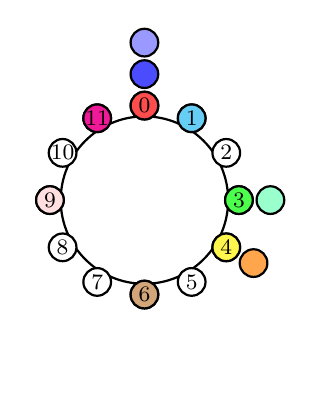
\begin{tikzpicture}[node distance =15em, >=stealth, ->, thick] 
			\node[circle, minimum size =6.05em, draw, thick] (C){};
			\foreach \i in {0, ..., 11}\node[circle, minimum size
			=1em, draw, fill=white, thick]at(\i*30: 1.2) (\i){};
			\node[circle, minimum size =1em, fill=red!70, draw, thick]at(3*30: 1.2) (r1){};
			\node[circle, minimum size =1em, fill=blue!70, draw, thick]at(3*30: 1.6) (r2){};
			\node[circle, minimum size =1em, fill=blue!40, draw, thick]at(3*30: 2) (r3){};
			\node[circle, minimum size =1em, fill=cyan!60, draw, thick]at(2*30: 1.2) (r4){};
			\node[circle, minimum size =1em, fill=green!70, draw, thick]at(0*30: 1.2) (r5){}; 
			\node[circle, minimum size =1em, fill=SpringGreen!40, draw, thick]at(0*30: 1.6) (r6){};
			\node[circle, minimum size =1em, fill=yellow!70, draw, thick]at(11*30: 1.2) (r7){}; 
			\node[circle, minimum size =1em, fill=orange!70, draw, thick]at(11*30: 1.6) (r8){};
			\node[circle, minimum size =1em, fill=brown!70, draw, thick]at(9*30: 1.2) (r9){};
			\node[circle, minimum size =1em, fill=pink!50, draw, thick]at(6*30: 1.2) (r10){};
			\node[circle, minimum size =1em, fill=magenta!90, draw, thick]at(4*30: 1.2) (r11){};
						
			\foreach \i in {0, ..., 11}\node[circle, minimum size
			=1em]at(90 - \i*30: 1.2) (pos){\footnotesize{\i}};
			\node[]at(9*30: 2) (181){\large{$~$}}; 
			\end{tikzpicture}
	}\hspace{1em}
	\subfloat[][
	]{
\centering 
			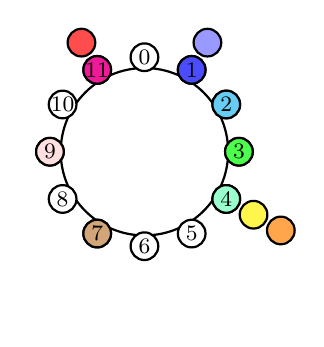
\begin{tikzpicture}[node distance =15em, >=stealth, ->, thick] 
			\node[circle, minimum size =6.05em, draw, thick] (C){};
			\foreach \i in {0, ..., 11}\node[circle, minimum size
			=1em, draw, fill=white, thick]at(\i*30: 1.2) (\i){};
			\node[circle, minimum size =1em, fill=red!70, draw, thick]at(4*30: 1.6) (r1){};
			\node[circle, minimum size =1em, fill=blue!70, draw, thick]at(2*30: 1.2) (r2){};
			\node[circle, minimum size =1em, fill=blue!40, draw, thick]at(2*30: 1.6) (r3){};
			\node[circle, minimum size =1em, fill=cyan!60, draw, thick]at(1*30: 1.2) (r4){};
			\node[circle, minimum size =1em, fill=green!70, draw, thick]at(0*30: 1.2) (r5){}; 
			\node[circle, minimum size =1em, fill=SpringGreen!40, draw, thick]at(11*30: 1.2) (r6){};
			\node[circle, minimum size =1em, fill=yellow!70, draw, thick]at(11*30: 1.6) (r7){}; 
			\node[circle, minimum size =1em, fill=orange!70, draw, thick]at(11*30: 2) (r8){};
			\node[circle, minimum size =1em, fill=brown!70, draw, thick]at(8*30: 1.2) (r9){};
			\node[circle, minimum size =1em, fill=pink!50, draw, thick]at(6*30: 1.2) (r10){};
			\node[circle, minimum size =1em, fill=magenta!90, draw, thick]at(4*30: 1.2) (r11){};
						
			\foreach \i in {0, ..., 11}\node[circle, minimum size
			=1em]at(90 - \i*30: 1.2) (pos){\footnotesize{\i}};
			\node[]at(9*30: 2) (181){\large{$~$}};			
			\end{tikzpicture}
	}\hspace{1em}
	\subfloat[][
	]{
\centering 
			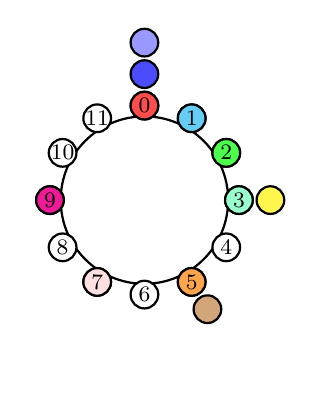
\begin{tikzpicture}[node distance =15em, >=stealth, ->, thick] 
			\node[circle, minimum size =6.05em, draw, thick] (C){};
			\foreach \i in {0, ..., 11}\node[circle, minimum size
			=1em, draw, fill=white, thick]at(\i*30: 1.2) (\i){};
			\node[circle, minimum size =1em, fill=red!70, draw, thick]at(3*30: 1.2) (r1){};
			\node[circle, minimum size =1em, fill=blue!70, draw, thick]at(3*30: 1.6) (r2){};
			\node[circle, minimum size =1em, fill=blue!40, draw, thick]at(3*30: 2) (r3){};
			\node[circle, minimum size =1em, fill=cyan!60, draw, thick]at(2*30: 1.2) (r4){};
			\node[circle, minimum size =1em, fill=green!70, draw, thick]at(1*30: 1.2) (r5){}; 
			\node[circle, minimum size =1em, fill=SpringGreen!40, draw, thick]at(0*30: 1.2) (r6){};
			\node[circle, minimum size =1em, fill=yellow!70, draw, thick]at(0*30: 1.6) (r7){}; 
			\node[circle, minimum size =1em, fill=orange!70, draw, thick]at(10*30: 1.2) (r8){};
			\node[circle, minimum size =1em, fill=brown!70, draw, thick]at(10*30: 1.6) (r9){};
			\node[circle, minimum size =1em, fill=pink!50, draw, thick]at(8*30: 1.2) (r10){};
			\node[circle, minimum size =1em, fill=magenta!90, draw, thick]at(6*30: 1.2) (r11){};
						
			\foreach \i in {0, ..., 11}\node[circle, minimum size
			=1em]at(90 - \i*30: 1.2) (pos){\footnotesize{\i}};
			\node[]at(9*30: 2) (181){\large{$~$}};			
			\end{tikzpicture}
	}
	\hspace{1em}
	\captionsetup[subfloat]{labelformat=empty}
	\subfloat[Legend][
	]{
			\centering 
			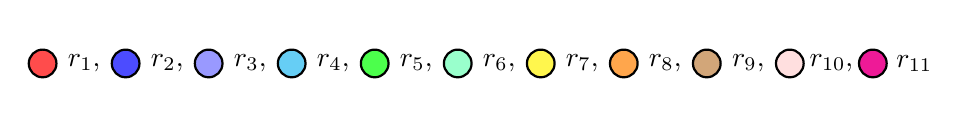
\begin{tikzpicture}[node distance =1.5em, >=stealth, ->, thick] 
			\node[circle, minimum size =1em, draw, fill=red!70, thick] (1){};
			\node[circle, minimum size =1em, right of = 1] (11){$r_1$, };
			\node[circle, minimum size =1em, draw, fill=blue!70, thick, right of = 11] (2){};
			\node[circle, minimum size =1em, right of = 2] (21){$r_2$, };
			\node[circle, minimum size =1em, draw, fill=blue!40, thick, right of = 21] (3){};
			\node[circle, minimum size =1em, right of = 3] (31){$r_3$, };
			\node[circle, minimum size =1em, draw, fill=cyan!60, thick, right of = 31] (4){};
			\node[circle, minimum size =1em, right of = 4] (41){$r_4$, };
			\node[circle, minimum size =1em, draw, fill=green!70, thick, right of = 41] (5){};
			\node[circle, minimum size =1em, right of = 5] (51){$r_5$, };
			\node[circle, minimum size =1em, draw, fill=SpringGreen!40, thick, right of = 51] (6){};
			\node[circle, minimum size =1em, right of = 6] (61){$r_6$, };
	
			\node[circle, minimum size =1em, draw, fill=yellow!70, thick, right of = 61] (7){};
			\node[circle, minimum size =1em, right of = 7] (71){$r_7$, };
			\node[circle, minimum size =1em, draw, fill=orange!70, thick, right of = 71] (8){};
			\node[circle, minimum size =1em, right of = 8] (81){$r_8$, };
			\node[circle, minimum size =1em, draw, fill=brown!70, thick, right of = 81] (9){};
			\node[circle, minimum size =1em, right of = 9] (91){$r_9$, };
			\node[circle, minimum size =1em, draw, fill=pink!50, thick, right of = 91] (10){};
			\node[circle, minimum size =1em, right of = 10] (101){$r_{10}$, };
			\node[circle, minimum size =1em, draw, fill=magenta!90, thick, right of = 101] (11){};
			\node[circle, minimum size =1em, right of = 11] (111){$r_{11}$};
			\end{tikzpicture}
	}\caption{Example of a $V_a$ to $V_p$ transition from $a$ to $b$, normalized in $c$.}
	\label{fig:ex: vaAsync}
\end{figure}
\end{example}
 %\todo{a need for fairness:  by fairness we mean that the scheduler always schedule at least one robot whose $\LC$ phase leads to any state that is not $\still$  or whose movement is not $\still$.}

%\todo{pas d'outils pour fairness in synthesis}
%\todo{explosion de l'espace d'état}

Given an adversary vertex $v = \bigl (o, \mem, (a_1, \dots, a_k)\bigr ) \in V_a$ and a player vertex $v' \in V_p$.
The edge $(v, v')$ belongs to $E$ if and only if there exists a non empty 
 subset $\Sched$ of $\Rob$, a $(v, \Sched)$-consistent state $\mem'$ and 
 a $(v, \Sched)$-move $m$ such that $v'=\bigl (\equivclass{o\oplus m}, \hat{\mem}' \bigr )$
 where $\hat{\mem}'$ has been obtained by normalizing $s'$.
%\todo{faire un dessin de l'arène avec observation partielle pour le player}


		\section {An algorithm for asynchronous synthesis}
In order to fight the combinatorial explosion due to the asynchronous model
we propose a method to obtain a gathering protocol in the asynchronous model 
combining synchronous synthesis and model-checking. 

We know that all executions in the synchronous model are also executions of the 
asynchronous models, then if a protocol is correct under the asynchronous 
execution model it is also correct under the synchronous model. Conversely, if a
protocol is not correct under the synchronous model it cannot be correct under 
the asynchronous one.
Thus, we use synchronous algorithm synthesis coupled with model-checking 
on the resulting strategy of the synthesis in an asynchronous execution model. 
If the strategy is correct then we have the desired protocol
 otherwise we search for a distinct synchronous strategy.
 
The Algorithm~\ref{algoSynth} takes as input the arena for ring size $n$ and $k$ robots. 
It constructs a tree of all synchronous strategies for the gathering and tests each one by model-checking in the asynchronous setting.
If an asynchronous strategy achieves the gathering then the tree construction is stopped.
 
 \begin{algorithm}
%\TitleOfAlgo{AsynchronousSynthesis} %%% redondant vec setAlgoRefName 
\SetAlgoRefName{AsyncSynth}
\AlgoDisplayBlockMarkers\SetAlgoBlockMarkers{}{}%: =:  ;
\SetAlgoNoEnd
\SetStartEndCondition{ }{}{}%
\SetKwProg{Fn}{Function}{\string: }{}
 \DontPrintSemicolon
\SetKwFunction{algo}{AsyncSynth}
\SetKwFunction{SS}{SS}
\Fn(\tcc*[h]{call to synchronous synthesis:  asking for a strategy that does not contain any rule of the CrList list}){\SS{CrList}}{
  \KwResult{A strategy as a rule list, if there is none it returns the empty List $\emptyset$}
}\BlankLine
%MC
\SetKwFunction{MC}{MC}
\Fn(\tcc*[h]{call to model checking on the algorithm composed of the rule list CrList in asynchronous model}){\MC{CrList}}{
  \KwResult{true or false}
}\BlankLine

\newcommand{\forcond}{$i=0$ \KwTo CurrentProc.size()-1 } 
\SetKwProg{Fn}{Function}{\string: }{}
\SetKwFunction{AS}{AsyncSynth}
\Fn(\tcc*[h]{The recursive function that calls synchronous synthesis and asynchronous  model-checking}){\AS{CrList L}}{
	\KwData{	CrList CurrentProc \;}
  	\KwResult{An algorithm as a List of Rules or $\emptyset$}
	CurrentProc = \SS{L}\;
	\eIf{isEmpty(CurrentProc)}
		{\Return $\emptyset$\;}
		{\eIf {\MC{CurrentProc}}
			{\Return CurrentProc \;}
			{\For{\forcond}{
				%pas besoin du test sur la profondeur ... dans ce coup de temps là il n'y a juste pas de solution
				CrList L' = L + CurrentProc[i] \;
				CrList Proc = \AS{L'}\;
				\If {not isEmpty(Proc)}
					{\Return Proc\;}
				%pas de else 
			}
			}
			%si tous les fils ont été vu alors on retourne $\emptyset$\;
			\Return $\emptyset$\;
		}	
}\BlankLine \BlankLine
 
  \SetKwProg{myalg}{Algorithm}{}{}
  \myalg{\algo{}}{
  \KwData{	Int n, k:  the size of the ring and the number of robots\;}
  \KwResult{A correct by construction algorithm as a List of Rules or $\emptyset$}
\Return{\AS{$\emptyset$}}
}

\caption{\label{algoSynth}}
\end{algorithm}


Each node of the tree is labeled by a strategy $\dec=(\dec_1, \dec_2, \dots, \dec_{|O|})$ where for each $i$, $\dec_i$ is the set 
of actions associated with the $i^{th}$ observation class, one action for each robot view.
The root of the tree is the strategy $\dec_{init}$ resulting from the call $SS(\emptyset)$, 
where no rule is forbidden.
A node of the tree is labeled by a strategy $\dec=(\dec_1, \dec_2, \dots, \dec_{|O|})$ resulting from some call 
$SS(L)$, where $L$ is the list of rules forbidden in $\dec$. This node has as many children 
as the number of observation classes, where the label of the $i^{th}$ child is the strategy denoted by $\dec^i$,  resulting from the call 
$SS(L \cup \{\dec_i\})$.

\begin{landscape}
\begin{example}
The Algorithm~\ref{algoSynth} builds a tree of all possible synchronous strategies until it finds one
that also achieve the gathering in the asynchronous execution model. 
Figure~\ref{fig:tree} represents one of the possible trees constructed by the algorithm
(depending on the synthesis function) for 2 robots 
%(noted respectively $m_1$ and $m_2$) 
in a ring where there are only three observation classes
and two possible strategies (in $\{0, 1\}$) in each configuration class. 
%(noted $C_1$, $C_2$, and $C_3$). 
In this example, we assume that every strategy achieves the gathering in a synchronous
setting but not in an asynchronous one, which permits to build the complete tree of synchronous strategies. 
A strategy is written as a word $\dec_1\dec_2\dec_3$, where $\dec_i$ is a binary digit representing the
strategy in the $i^{th}$ class of observations. 
\begin{figure}
\centering 
\scriptsize
\begin{forest}
for tree={ellipse, draw, l sep=20pt}
[000%, red 
	[111
		[$\emptyset$]
		[100
			[$\emptyset$]
			[$\emptyset$]
			[101
				[$\emptyset$]
				[$\emptyset$]
				[$\emptyset$]
			]
		]
		[100
			[$\emptyset$]
			[110
				[$\emptyset$]
				[$\emptyset$]
				[$\emptyset$]
			]
			[$\emptyset$]
		]
	]
	%mid
    	[111, red
      		[010, blue
			[$\emptyset$]
			[$\emptyset$]
			[011, green
				[$\emptyset$]
				[$\emptyset$]
				[$\emptyset$]
			]
		] 
      		[$\emptyset$] 
      		[110
			[010
				[$\emptyset$]
				[$\emptyset$]
				[$\emptyset$]
			]
			[$\emptyset$]
			[$\emptyset$]
		]
  	]
	%end
	[111
		[001
			[$\emptyset$]
			[011
				[$\emptyset$]
				[$\emptyset$]
				[$\emptyset$]
			]
			[$\emptyset$]
		]
		[101
			[001
				[$\emptyset$]
				[$\emptyset$]
				[$\emptyset$]
			]
			[$\emptyset$]
			[$\emptyset$]
		]
		[$\emptyset$]
	]
]
\end{forest}
	\caption{Example of a tree constructed by \ref{algoSynth}}
	\label{fig:tree}
\end{figure}
The root of the tree corresponds to the strategy returned by the function $SS(\emptyset)$.
The red, blue and green nodes correspond respectively to the strategies given by $SS(\sigma_2 = 1)$, 
$SS(\sigma_2 = 1, \sigma_1 = 0)$ and $SS(\sigma_2 = 1, \sigma_1 = 0, \sigma_3 = 0)$.
\end{example}
\end{landscape}

If there is no synchronous strategy that performs the gathering in the asynchronous model, 
then it means that no protocol exists for this model.
Moreover, if there is a gathering protocol our algorithm will find it.

\begin{lemma}
\label{algoEnd}
The Algorithm~\ref{algoSynth} terminates.
\end{lemma}
\begin{proof}
Since the size of the ring and the number of robots are known and finite, the number of configuration classes is known 
and finite (note that this would also be the case for any other finite graph). 
The number of strategies is then bounded by $|\Actions|^{k |O|}$.
At each step the algorithm increments the number of different forbidden rules, and thus decrement the number of strategies. 
If no asynchronous protocol is found the number of forbidden rules  for an observation class will be equal to
the number of possible strategies for this class, hence there is no more synchronous strategy and 
thus the algorithm terminates.
\end{proof}

\begin{lemma}
\label{algoCompletness}
The Algorithm~\ref{algoSynth} is complete.
\end{lemma}
\begin{proof}
%The algorithm is complete because any protocol achieving asynchronous gathering will be found.
To show that the algorithm is complete, we proceed by contradiction. Assume that the algorithm cannot find 
an existing asynchronous gathering protocol. This means that every leaf of the tree is $\emptyset$, hence 
at least one rule of the protocol is forbidden in each leaf, thus
these rules were present in the leaf's ancestors.
Assume that the algorithm is currently building node $x$ and that no rule of the protocol is forbidden in this step, but 
none of its subtrees contains the protocol. 
If none of its subtrees contains the protocol, it means that at least one rule of the protocol is forbidden
in every child.
If a rule is forbidden in a child and not in its parent it means that the parent strategy contains this rule.
%Since in $x$ no rule of the protocol is forbidden and yet none of its child contains the protocol
Then the node $x$ must contain the protocol, hence we have a contradiction.
\end{proof}

\begin{theorem}
There is a gathering protocol if and only if Algorithm~\ref{algoSynth} returns a non empty list.
\end{theorem}

\begin{proof}
The algorithm is correct since it terminates (Lemma~\ref{algoEnd}), it is correct because any protocol produced by the synthesis (Theorem~\ref{th: correctness}) is tested by model checking and hence is a solution to asynchronous gathering, and it is complete (Lemma~\ref{algoCompletness}).
\end{proof}

















